%%%%%%%%%%%%%%%%%%%%%%%%%%%%%%%%%%%%%%%%%
% kaobook
% LaTeX Template
% Version 1.3 (December 9, 2021)
%
% This template originates from:
% https://www.LaTeXTemplates.com
%
% For the latest template development version and to make contributions:
% https://github.com/fmarotta/kaobook
%
% Authors:
% Federico Marotta (federicomarotta@mail.com)
% Based on the doctoral thesis of Ken Arroyo Ohori (https://3d.bk.tudelft.nl/ken/en)
% and on the Tufte-LaTeX class.
% Modified for LaTeX Templates by Vel (vel@latextemplates.com)
%
% License:
% CC0 1.0 Universal (see included MANIFEST.md file)
%
%%%%%%%%%%%%%%%%%%%%%%%%%%%%%%%%%%%%%%%%%

%----------------------------------------------------------------------------------------
%	PACKAGES AND OTHER DOCUMENT CONFIGURATIONS
%----------------------------------------------------------------------------------------

\documentclass[
	a4paper, % Page size
	fontsize=10pt, % Base font size
	twoside=true, % Use different layouts for even and odd pages (in particular, if twoside=true, the margin column will be always on the outside)
	%open=any, % If twoside=true, uncomment this to force new chapters to start on any page, not only on right (odd) pages
	%chapterentrydots=true, % Uncomment to output dots from the chapter name to the page number in the table of contents
	numbers=noenddot, % Comment to output dots after chapter numbers; the most common values for this option are: enddot, noenddot and auto (see the KOMAScript documentation for an in-depth explanation)
]{kaobook}

% Choose the language
\ifxetexorluatex
	\usepackage{polyglossia}
	\setmainlanguage{italian}
\else
	\usepackage[italian]{babel} % Load characters and hyphenation
\fi

% Load packages for testing
\usepackage{blindtext}
%\usepackage{showframe} % Uncomment to show boxes around the text area, margin, header and footer
%\usepackage{showlabels} % Uncomment to output the content of \label commands to the document where they are used

% Load the bibliography package
\usepackage{kaobiblio}
\addbibresource{main.bib} % Bibliography file

% Load mathematical packages for theorems and related environments
\usepackage[framed=true]{kaotheorems}

% Load the package for hyperreferences
\usepackage{kaorefs}

\usepackage{csquotes}

\usepackage{algorithm2e}

\graphicspath{{examples/documentation/images/}{images/}} % Paths in which to look for images

\makeindex[columns=3, title=Alphabetical Index, intoc] % Make LaTeX produce the files required to compile the index

% \makeglossaries % Make LaTeX produce the files required to compile the glossary
% \newglossaryentry{computer}{
	name=computer,
	description={is a programmable machine that receives input, stores and manipulates data, and provides output in a useful format}
}

% Glossary entries (used in text with e.g. \acrfull{fpsLabel} or \acrshort{fpsLabel})
\newacronym[longplural={Frames per Second}]{fpsLabel}{FPS}{Frame per Second}
\newacronym[longplural={Tables of Contents}]{tocLabel}{TOC}{Table of Contents}

 % Include the glossary definitions

%\makenomenclature % Make LaTeX produce the files required to compile the nomenclature

% Reset sidenote counter at chapters
%\counterwithin*{sidenote}{chapter}


%----------------------------------------------------------------------------------------

\begin{document}

%----------------------------------------------------------------------------------------
%	BOOK INFORMATION
%----------------------------------------------------------------------------------------

% \titlehead{The \texttt{kaobook} class}
% \subject{Use this document as a template}

\title[Elaborato di Fisica Computazionale]{Elaborato di Fisica Computazionale}
\subtitle{A.A 2024/2025}

\author[Andrea Rossi]{Andrea Rossi \xspace \texttt{N. 897139}}

% \date{\today}

%----------------------------------------------------------------------------------------

\frontmatter % Denotes the start of the pre-document content, uses roman numerals

%----------------------------------------------------------------------------------------
%	OPENING PAGE
%----------------------------------------------------------------------------------------

\iffalse
\makeatletter
\extratitle{
	% In the title page, the title is vspaced by 9.5\baselineskip
	\vspace*{9\baselineskip}
	\vspace*{\parskip}
	\begin{center}
		% In the title page, \huge is set after the komafont for title
		\usekomafont{title}\huge\@title
	\end{center}
}
\makeatother
\fi

%----------------------------------------------------------------------------------------
%	OUTPUT TITLE PAGE AND PREVIOUS
%----------------------------------------------------------------------------------------

% Note that \maketitle outputs the pages before here

\maketitle

%----------------------------------------------------------------------------------------
%	PREFACE
%----------------------------------------------------------------------------------------

\chapter*{Prefazione}
\addcontentsline{toc}{chapter}{Preface} % Add the preface to the table of contents as a chapter

Nel seguente elaborato verrà illustrata l’analisi degli argomenti proposti nel
corso di Fisica Computazionale.

Di seguito sono riportate le informazioni richieste per una fruizione completa 
del documento:

	\paragraph{Codice sorgente e dati} Il codice sorgente ed i dati analizzati nei 
        vari esercizi sono reperibili al seguente 
        \href{https://github.com/ARossiUnimib/Fisica-Computazionale}{repository Github} 
        nelle cartelle dei capitoli omonimi.

	\paragraph{Lingua del codice} La lingua utilizzata nel codice sorgente sarà 
        l’inglese per avere una maggiore coesione sintattica con i linguaggi di 
        programmazione utilizzati, la spiegazione generale del codice sarà presente
        nell'elaborato, per ulteriori informazioni riferirsi alla documentazione,
        presente nel repository.

	\paragraph{Introduzione dei moduli} Verranno ripetute, sopratutto nella parte 
        introduttiva dei vari capitoli, i punti chiave recuperati dalle risorse 
        disponibili sull’e-learning del corso. 
        Esse saranno riassuntive favorendo le precisazioni e lo studio
		degli esercizi per ottenere un quadro completo dei vari argomenti.


\index{preface}

%----------------------------------------------------------------------------------------
%	TABLE OF CONTENTS & LIST OF FIGURES/TABLES
%----------------------------------------------------------------------------------------

\begingroup % Local scope for the following commands

% Define the style for the TOC, LOF, and LOT
\setstretch{1} % Uncomment to modify line spacing in the ToC
%\hypersetup{linkcolor=blue} % Uncomment to set the colour of links in the ToC
\setlength{\textheight}{230\hscale} % Manually adjust the height of the ToC pages


% Turn on compatibility mode for the etoc package
\etocstandarddisplaystyle % "toc display" as if etoc was not loaded
\etocstandardlines % "toc lines" as if etoc was not loaded

\tableofcontents % Output the table of contents

%\listoffigures % Output the list of figures

% Comment both of the following lines to have the LOF and the LOT on different pages
\let\cleardoublepage\bigskip
\let\clearpage\bigskip

% \listoftables % Output the list of tables

\endgroup

%----------------------------------------------------------------------------------------
%	MAIN BODY
%----------------------------------------------------------------------------------------

\mainmatter % Denotes the start of the main document content, resets page numbering and uses arabic numbers
\setchapterstyle{kao} % Choose the default chapter heading style

\setchapterpreamble[u]{\margintoc}
\chapter{Numeri}
\labch{numbers}

\section{Rappresentazione}

La rappresentazione numerica a cui il calcolo scientifico fa riferimento principalmente
è quella dei numeri reali; nell’ambito informatico tale rappresentazione utilizza
il concetto di numeri a virgola mobile come standard: i numeri reali vengono
rappresentati attraverso una notazione scientifica in base due tramite la seguente formula:

$$
	(-1)^S \left( 1 + \sum_n M_n 2^{-n} \right) \cdot 2^{E}
$$

Dove:
\begin{description}
	\item $S$ è il valore booleano per il \textbf{segno}
	\item $M$ è la parte decimale detta \textbf{mantissa}

	\item $E = e - d$ è l'\textbf{esponente} con $d$ (offset), $e$ (esponente dopo offset)
\end{description}

\section{Esercizi}

\subsection{Precisione}

\paragraph{Nozioni teoriche}

\subparagraph{Definizione} La \textit{precisione di macchina} (o \textit{$\epsilon$ di macchina})
è la differenza tra 1 e il numero successivo rappresentabile dato il numero di bit
richiesti, esso sarà dunque:

$$
	\epsilon = 2^{-M}
$$

Nello standard dei numeri a virgola mobile (IEE 754) si studiano principalmente
due sottoclassi di numeri i cui nominativi nei linguaggi C-like sono:

\begin{description}
	\item[float] numero a singola precisione (32 bit di memoria):
		\begin{itemize}
			\item $M$: 23 bit
			\item $E$: 8 bit
			\item Valore massimo: $3.40 \cdot 10^{38}$
			\item $\epsilon$: $\sim 10^{-7}$
		\end{itemize}
	\item[double] numero a doppia precisione (64 bit di memoria):
		\begin{itemize}
			\item $M$: 52 bit
			\item $E$: 11 bit
			\item Valore massimo: $1.8 \cdot 10^{308}$
			\item $\epsilon$: $\sim 10^{-16}$
		\end{itemize}

\end{description}

\paragraph{Richiesta} Scriverete un programma C che esegua le seguenti operazioni:

\begin{lstlisting}
    define f in single precision = 1.2e34
    for loop with 24 cycles:
        f *= 2
        print f in scientific notation
    repeat for d in double precision, starting from 1.2e304
    define d in double precision = 1e-13
    for loop with 24 cycles:
        d /= 2
        print d and 1+d in scientific notation
    repeat for single precision
\end{lstlisting}

Esaminare il range minimo e massimo e il ruolo dell'errore di macchina.

\paragraph{Implementazione e osservazioni}

\subparagraph{File necessari} sorgente: \texttt{number\_precision.c}, dati: \texttt{number\_precision.dat}

Il codice sorgente scritto utilizza funzionalità base del linguaggio C. \sidenote{
	Per formattare il codice secondo la richiesta del problema si usi la
	definizione \texttt{EXERCISE\_FORMAT}, altrimenti verrà utilizzata una formattazione
	più compatta per leggere in maniera più diretta i dati, si consiglia di utilizzare
	quest'ultima per comprendere l'analisi sottostante}

\paragraph{Analisi e conclusioni}

Dai dati ottenuti si possono notare in maniera esaustiva varie proprietà dei
numeri a virgola mobile:

\begin{enumerate}
	\item Esiste un \textit{valore massimo} sia per singola ($\sim 3 \cdot 10^{38}$) sia
	      per doppia precisione ($\sim 2 \cdot 10^{308}$), superato esso viene mostrato un
	      valore esatto \textit{inf} definito dallo standard descritto in precedenza;

	\item I numeri hanno un \textit{errore macchina} dettato dalla capienza di memoria della mantissa;

	\item Come mostrerà più precisamente la prossima sezione, l’errore viene
	      \textit{propagato} nella somma:

	      \begin{itemize}
		      \item $1 + f_{mult}$ perde completamente l’informazione su $f_{mult}$

		      \item $1 + d_{mult}$ la conserva soltanto per le prime iterazioni;
	      \end{itemize}
\end{enumerate}
\subsection{Propagazione degli errori}
\paragraph{Nozioni teoriche}

E' immediato notare come i numeri a virgola mobile possano essere rappresentati come
variaili casuali con errore associato, derivante dalla precisione di macchina.

Prendiamo in esame una funzione $f(x, y)$ dove $x, y$ sono variabili casuali indipendenti
con rispettivo errore $\sigma_x, \sigma_y$, allora l'errore su f sarà:

$$
	\sigma_f^2 = {\left( \frac{\partial f}{\partial x} \right)^2 \sigma_x^2 + \left( \frac{\partial f}{\partial y} \right)^2 \sigma_y^2}
$$

Assumendo ora $f = x + y$ otteniamo:

$$
	\sigma_f^2 = {\sigma_x^2 + \sigma_y^2}
$$

Notiamo immediatamente quindi che se $x \gg y $ allora $\sigma_f \approx \sigma_x$ quindi
si perde l'informazione su $y$ nella somma.


\paragraph{Richiesta} 

Si scriva in C un programma che esegua le seguenti operazioni:

\begin{lstlisting}
    calculate (0.7 + 0.1) + 0.3 and print 16 digits
    calculate 0.7 + (0.1 + 0.3) and print 16 digits
    define xt = 1.e20; yt = -1.e20; zt = 1
    calculate (xt + yt) + zt
    calculate xt + (yt + zt)
\end{lstlisting}

Esaminare la non-associatività dell'addizione e il ruolo degli errori di arrotondamento.



\paragraph{Implementazione e osservazioni}

\subparagraph{File necessari} sorgente: \texttt{error\_propagation.c}

In base alle richieste l'output è il seguente:

\begin{enumerate}

	\item $(0.7 + 0.1) + 0.3 =_? 0.7 + (0.1 + 0.3)$:
	      $$\texttt{Output: 1.1000000238418579, 1.1000000238418579}$$

	      La somma risulta associativa.

	\item $[10^{20} + (-10^{20})] + 1 =_? 10^{20} + [(-10^{20}) + 1]$:
	      $$\texttt{Output: 1.0000000000000000, 0.0000000000000000}$$

	      La somma risulta non associativa.
\end{enumerate}

\label{sec:propagation}
\paragraph{Analisi}

Utilizzando le formule discusse si può studiare la propagazione dell’errore nella somma.
In essa la propagazione dipende dall’errore assoluto dei singoli addendi.
Assumendo numeri a singola precisione e ricordando che $ \sigma_x \approx \epsilon \sim 10^{-7}$,
si ottengono i seguenti casi:

\begin{enumerate}

	\item Per i valori 0.7, 0.1, 0.3 l’ordine di grandezza è lo stesso, quindi,
	      tutti i valori possegono un errore assoluto $\Delta x \sim 10^{-8}$; propagando
	      l’errore nella somma si ottiene dunque $\Delta_{output} \sim 3 \cdot \Delta x$ in accordo con
	      i risultati.

	\item Il risultato è describile come un caso limite nell’errore di propagazione rispetto
	      alla singola precisione, infatti, $10^{20}$ avrà un errore assoluto di $\sim 10^{13}$
	      mentre 1 di $10^{-7}$!

	      La spiegazione dell'output ottenuto, dunque, si basa sulla differenza
	      tra ordini di grandezza dei diversi addendi:
	      \begin{itemize}
		      \item Nel termine a sinistra
		            vengono sommati prima numeri con errore assoluto paragonabile.
		            Si ottiene quindi $\sim 0$ che sarà poi sommato con un numero
		            avente errore assoluto simile a 1.

		      \item
		            Nel termine a destra, invece, si sommano due valori con venti
		            ordini di grandezza di differenza: l’errore assoluto di
		            $10^{20}$ prevale e si perde qualsiasi informazione nella somma per termini:
		            $$x \ll 10^{20} \Rightarrow x + 10^{20} \sim 10^{20}$$
		            Segue che $\mathit{1}$ sarà ignorato nella somma a destra.
	      \end{itemize}

\end{enumerate}

\paragraph{Conclusioni}
Nel manipolare numeri in un calcolatore l’operazione eseguita, la precisione e
la differenza in ordine di grandezza dei numeri partecipanti devono essere tenuti
sempre in considerazione specialmente nelle addizioni.



\setchapterpreamble[u]{\margintoc}
\chapter{Matrici}
\labch{matrices}

\section{Introduzione}

\paragraph{Struttura del codice}

Da questo capitolo in poi, il codice sorgente utilizzera come linguaggio primario
C++. La librerie necessarie prima di proseguire sono le seguenti:

\begin{itemize}
    \item \texttt{tensor.hpp} versione modificata di \texttt{matrix.h} disponibile
        su e-learning: l'header e' stato generalizzato per funzionare sia come
        vettori sia come matrici rendendo le operazioni compatibili fra i due e 
        facilitando il successivo svolgimento degli esercizi.
    \item \texttt{tensor\_utils.hpp} contentente varie funzionalita' utili e contente
        gli argomenti creati per ogni esercizio
    
\end{itemize}

\section{Esercizi}

\subsection{Inversione di matrici triangolari}

\subsection{Eliminazione di Gauss}

\subsection{Decomposizione LU}



\setchapterpreamble[u]{\margintoc}
\chapter{Intepolazione}
\labch{interp}

\section{Esercizi}

\subsection{Interpolazione}

\subsection{Funzione di Runge}

\subsection{Esercizio 3?}


\setchapterpreamble[u]{\margintoc}
\chapter{Autovalori e autovettori}
\labch{eigenvalues}

\section{Introduzione ed esercizio 8}

\subparagraph{File necessari} \texttt{eigenvalues.hpp}

\subparagraph{Esercizio}

Per illustrare esaustivamente le tecniche numeriche utilizzate si considerino i
vari punti dell'esercizio 8 partendo dalla matrice seguente:

\[ A = \begin{pmatrix}
		4 & -i   & 2    \\
		i & 2    & 2+7i \\
		2 & 2-7i & -2
	\end{pmatrix} \]

\section{Punto 1: Power method}

\paragraph{Nozioni teoriche}

Il primo metodo e' definito \textit{Power method} e consiste nel calcolare l'autovalore piu' grande di una matrice $A$ e l'autovettore associato.

Dato un qualsiasi vettore per il teorema spettrale se $A$ e' diagonalizzabile allora ogni vettore $\mathbf{x}_0$ puo' essere scritto sulla base dagli autovettori $\mathbf{v}_n$ di $A$.

Prendiamo dunque il vettore:

\[ \mathbf{y}_n = \mathbf{A}^n \mathbf{x}_0 = \sum_m^N c_m \lambda_m^n \mathbf{v}_m= \lambda_{max} \sum_m^N c_m \left( \frac{\lambda_m}{\lambda_{max}} \right)^n \mathbf{v}_m\]

Per numeri sufficientemente grandi di $N$ e se il rapporto $\frac{\lambda_m}{\lambda_{max}}$ e' minore di 1 allora il termine $\left( \frac{\lambda_m}{\lambda_{max}} \right)^n$ tende a 0 e quindi il termine dominante e' $\lambda_{max}$.

Quindi \[ \lim_{n \rightarrow \infty} \mathbf{y}_n = c_0 \lambda_{max} \mathbf{v}_0 \]

Visto che $\mathbf{y}_0$ e' multiplo di $\mathbf{v}_0$ esso stesso e' autovettore .

Per ottenere l'autovalore calcoliamo il cosiddetto \textit{Coefficiente di Rayleigh}

\[ \mathsf{C}_R = \frac{\mathbf{y}_n^T \mathbf{A} \mathbf{y}_n}{\mathbf{y}_n^T \mathbf{y}_n} \xrightarrow{n = \infty} \frac{\mathbf{v}_0^T \lambda_{max} \mathbf{v}_0}{\mathbf{v}_0^T \mathbf{v}_0} = \lambda_{max} \]

\subparagraph{Shifted Power Method}

Per casi particolari (principalmente autovalori simmetrici e opposti, come si vedra' nella ricerca degli zeri di polinomi ortonormali) si utilizza il \textit{Shifted Power Method}: si introduce uno shift $A + \alpha I$ per rendere lo spettro positivo e si reshiftano gli autovalori di $\lambda-\alpha$ ad algoritmo finito. Questo evita il carattere oscillatorio che si puo' estaurare quando $\lambda_i = -\lambda_j$.
In questo capitolo assumeremo $\alpha = 0$.

\paragraph{Implementazione}

La documentazione dell'algoritmo e' esaustiva e non necessita di ulteriori spiegazioni.

\paragraph{Risultati} si ottiene il seguente output:

\begin{lstlisting}
Power Eigenvalue: (8.45188,-2.22045e-16)
Power Eigenvector: 
 (0.387073,-0.143579)
 (0.350492,0.615922)
 (0.55364,-0.144353)

Ax= 
 (0.387073,-0.143579)
 (0.350492,0.615922)
 (0.55364,-0.144353)
\end{lstlisting}

Dove tra parentesi si indica la parte reale e immaginaria rispettivamente, inoltre il metodo funziona correttamente visto che $Ax = \lambda x$ ($\lambda$ e' molplicato nell'autovettore ma essendo una costante cio' e' ininfluente).

\section{Punto 2: Inverse Power method}

\paragraph{Nozioni teoriche}

Analogamente per il metodo precedente si puo' calcolare l'autovalore piu' piccolo di una matrice $A$ e l'autovettore associato, in questo caso si invertira' $A$e si raccogliera' il termine piu' piccolo $\lambda_{min}$ mentre $\left( \frac{\lambda_{min}}{\lambda_n} \right)^n \rightarrow 0$, lo stesso ragionamento si puo' anche fare per lo shift in questo caso esso verra' utilizzato per raggiungere piu' velocemente il risultato.

\paragraph{Risultati} Si ottiene:

\begin{lstlisting}
 Inverse Power Eigenvalue: (3.1896,-6.93889e-18)
Inverse Power Eigenvector: 
 (0.00850804,0.906366)
 (0.370705,-0.0809101)
 (0.0370076,-0.181906)

Ax= 
 (0.00850804,0.906366)
 (0.370705,-0.0809101)
 (0.0370076,-0.181906)
\end{lstlisting}

Il risultato e' inoltre verificato dal controllo di $\mathbf{Ax}$.

\section{Punto 3: studio della convergenza}

\paragraph{Risultati}


\begin{marginfigure}
	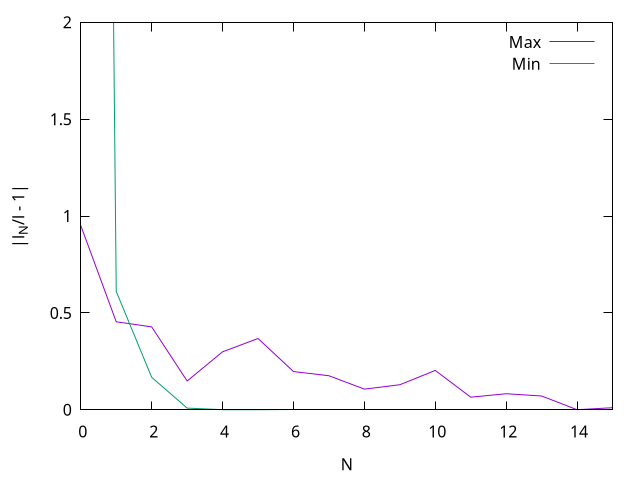
\includegraphics[width=1.5\textwidth]{eigen_convergence.png}
	\caption{Confronto tra la velocita' di convergenza dei due metodi}
	\label{fig:eigenconv}
\end{marginfigure}

Il risultato e' visibile nella figura \ref{fig:eigenconv}.

\paragraph{Analisi e conclusioni}

\begin{marginfigure}
	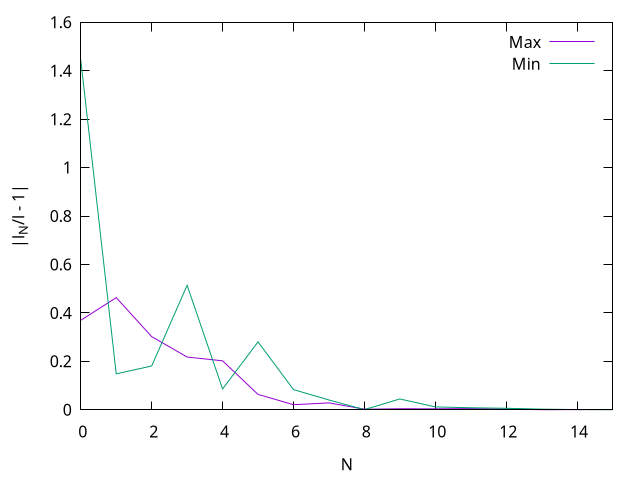
\includegraphics[width=1.5\textwidth]{eigen_convergence_2.png}
	\caption{Confronto tra la velocita' di convergenza dei due metodi, con $a_{00} = 8$}
	\label{fig:eigenconv_2}
\end{marginfigure}


Come si puo' osservare il metodo inverso converge molto piu' velocemente del
metodo diretto. Questo pero' dipende dagli autovalori della matrice e dal
rapporto $\lambda_n/\lambda_{max}$ e $\lambda_{min}/\lambda_n$. Per esempio,
presa la matrice A con $a_{00} = 8$ gli autovalori sono molto piu' vicini e si
ottiene la figura \ref{fig:eigenconv_2}.

\section{Punto 4: Deflation method}

\paragraph{Nozioni teoriche}

Attraverso l'utilizzo del \textit{Power method} possiamo inoltre ottenere tutti gli autovettori e autovalori di una matrice $A$ tramite il \textit{Deflation method}: trovato l'autovalore massimo possiamo rimuoverlo dallo spettro della matrice $A$ in questo modo otterremo il secondo valore massimo e cosi' via per tutti gli autovalori, ovviamente cio' non potrebbe funzionare nel caso del metodo inverso poiche', sottraendo l'autovalore alla matrice, otterremmo una matrice singolare e dunque non invertibile.

Per far cio' si puo' rimuovere iterativamente la proiezione di $\mathbf{v}_{0}$ corrente da $A$:

\[ A' = A - \lambda_{max} \mathbf{v}_{0} \mathbf{v}_{0}^T \]


\paragraph{Implementazione} In maniera simile alla precedente la documentazione e le funzione della classe \texttt{Tensor<T>} rendono l'implementazione triviale.

\paragraph{Risultati} Si ottengono i seguenti autovalori:

\begin{lstlisting}
(8.45188,0)
(-7.64148,0)
(3.1896,6.93889e-18)
\end{lstlisting}

Si nota banalmente che l'autovalore $\lambda_{min}$ corrisponde con quello trovato nel punto 2. Unica considerazione e' la parte immaginaria che in questo caso risulta 0 per l'autovalore massimo ma, essendo il valore precedente $< \epsilon_{double}$, si puo' considerare 0.






\setchapterpreamble[u]{\margintoc}
\chapter{Ricerca degli zeri}
\labch{zeri}
%NOTE: il risultato con Newton-Raphson puo' non convergere se la derivata e' nulla (punto stazionario o punto di flesso)

%NOTE: e' meglio combinare il metodo di bisezione con il metodo di Newton-Raphson: si fa qualche ciclo di bisezione e poi si utilizza il metodo di Newton

% |c-c_n| <= 2^{-n} |b-a|, |c-c_n+1| <= |c-c_n|
% scala logaritmica -> retta, algoritmi migliori

\section{Esercizi}

%TODO:

\subsection{Esercizio 9}

\begin{marginfigure}
	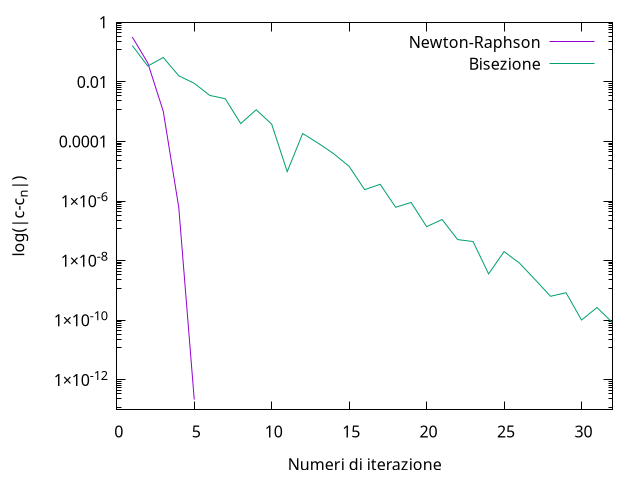
\includegraphics[width=1.5\textwidth]{roots_9_convergence_analysis.png}
	\caption{Convergenza dei due meetodi}
	\label{fig:roots_ex_9}
\end{marginfigure}

\begin{enumerate}
	\item Dato $-x^2 + x + \frac{1}{2} = 0$ le radici sono $x_{\pm}=\frac{-1 \pm \sqrt{1-4(-1)(1/2)}}{-2}=\frac{1\pm\sqrt{3}}{2}$. Dal metodo di bisezione otteniamo \texttt{1.36603} nell'intervallo $[0.8,1.6]$ come verificato dalla teoria, il medesimo risultato si ottiene per il metodo di Newton-Raphson.
	\item TODO:
    \item[3, 4] Dalla \reffig{roots_ex_9} si osserva che il metodo di bisezione converge piu' lentamente rispetto a quello di Newton-Raphson. Inoltre si osserva che il metodo di Bisezione converge linearmente ($\sim 2^{-n}$).
\end{enumerate}


\subsection{Esercizio 10}

\paragraph{Convergenza lenta} Lo zero della funzione $x^2$ e' banalmente $0$ se
consideriamo l'espressione analitica dell'errore del metodo di Newton-Raphson otteniamo: 
\[
    |0-x_{n+1}| = x_n - \frac{x_n^2}{2 x_n} = x_n - \frac{1}{2} x_n = \frac{1}{2}x_n
\]
Quindi l'errore del metodo di Newton-Raphson e' lineare in questo caso specifico.
In effetti come si puo' osservare dal file \texttt{ex\_10\_1.dat} si ottiene un valore costante di \texttt{0.5} come da teoria (a meno di errori di precisione successivi).

In conclusione la convergenza del metodo di Newton-Raphson, nonostante in generale sia quadratica, puo' essere diversa da quella prevista, a causa delle proprieta' analitiche della funzione in esame.

\paragraph{Cicli} 

Nei casi in cui si vuole studiare la convergenza del metodo di Newton-Raphson si
puo' studiare il frattale associato. Con un semplice programma python (\texttt{newton\_fractal.py}) si possono studiare le aree di convergenza del metodo data la
funzione.

TODO

\paragraph{Condizioni iniziali} Anche in questo caso studiamo i risultati e il
frattale associato alla funzione ottenendo \reffig{ex_10_3} e \reffig{newton_fractal_2}.

Dei valori iniziali relativamente simili cadono in delle regioni di convergenza 
diverse, basterebbe un leggero spostamento della condizione iniziale per ottenere uno zero differente.

Il carattere oscillatorio e' spiegabile analogamente al punto precedente.
\begin{marginfigure}
    \hspace{-2.1cm}
	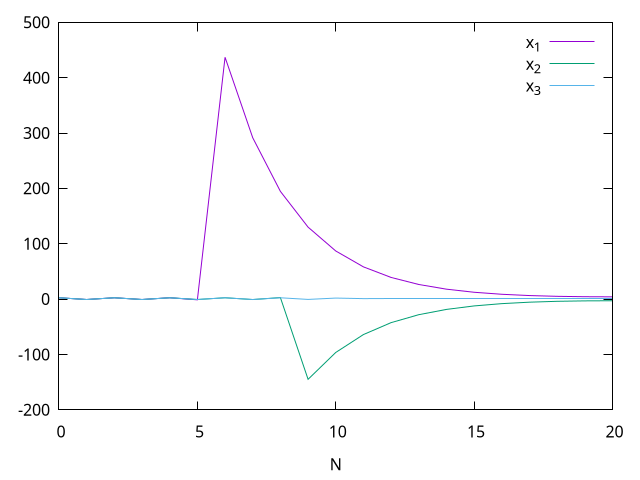
\includegraphics[width=1.5\textwidth]{initial_value_roots.png}
	\caption{Carattere oscillatorio del metodo di Newton per le condizioni iniziali del terzo punto, $x_1, x_2, x_3$ sono i valori in ordine proposti nelle note}
	\label{fig:ex_10_3}
\end{marginfigure}

\begin{marginfigure}
    \hspace{-2.1cm}
	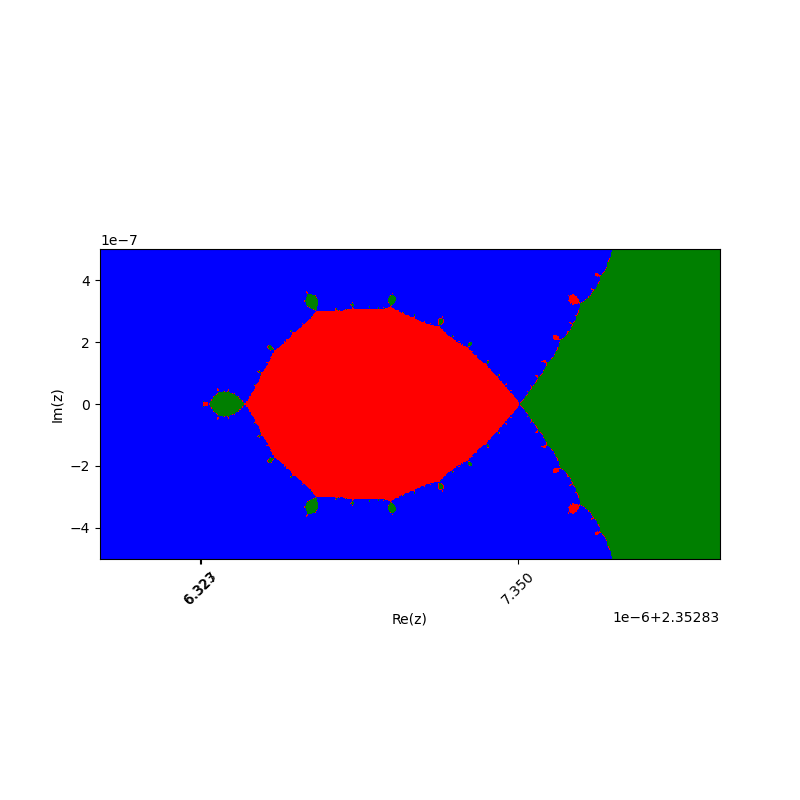
\includegraphics[width=1.5\textwidth]{newton_fractal.png}
	\caption{Frattale di Newton associato al terzo punto, colori diversi corrispondono a zeri diversi, si noti che due dei valori sono quasi sovrapposte in questa scala}
	\label{fig:newton_fractal_2}
\end{marginfigure}

\subsection{Esercizio 11}

\paragraph{Implementazione}

L'implmentazione e' diretta: 
\begin{lstlisting}[language=C++]
  // ... Asserts e definizione della funzione

  int n_coeffs = coefficients.Rows() - 1;

  auto coeffs_matrix = tensor::Tensor<T>::SMatrix(n_coeffs);

  // Si riempie la matrice 
  for (int i = 0; i < n_coeffs; i++) {
    if (i < n_coeffs - 1) {
      coeffs_matrix(i, i + 1) = 1.0;
    }

    coeffs_matrix(n_coeffs - 1, i) = -coefficients(i) / coefficients(n_coeffs);
  }

  // Si utilizza il Deflation Method con un termine correttivo alpha
  auto solution = eigen::PowerMethodDeflation(coeffs_matrix, n, alpha);

  // Sorting e return...
\end{lstlisting}

\paragraph{Analisi risultati}

Dopo aver aggiunto uno shift del \textit{Power method} rispettivamente di $\alpha_1=0.01, \alpha_2=0.1$. Si ottengono i seguenti valori

\begin{lstlisting}

\end{lstlisting}

\begin{minipage}{0.45\textwidth}
\lstset{basicstyle=\ttfamily\small, frame=single}
\begin{lstlisting}
Zeri di Legendre:
-0.973907
-0.865063
-0.67941
-0.433395
-0.148874
0.148874
0.433395
0.67941
0.865063
0.973907
Check:
2.59017e-07
4.42142e-08
-1.97815e-11
-5.12745e-11
7.348e-09
1.31299e-09
8.9706e-12
2.01226e-11
-4.42287e-08
-2.59039e-07
\end{lstlisting}
\end{minipage}
\hfill
\begin{minipage}{0.45\textwidth}
\lstset{basicstyle=\ttfamily\small, frame=single}
\begin{lstlisting}
Zeri di Hermite: 
-2.3506
-1.33585
0.00120427
0.436077
1.33585
2.3506
0.433395
-0.433395
0
7.16395e-322
Check:
1.81899e-12
-6.25278e-13
-119.999
-3.86358e-13
1.02318e-12
1.81899e-12
\end{lstlisting}
\end{minipage}

L'algoritmo funziona dunque correttamente.



\setchapterpreamble[u]{\margintoc}
\chapter{Equazioni differenziali ordinarie}
\labch{odes}

\section{Introduzione}

Un'equazione differenziale ordinaria (ODE) è un'equazione differenziale che
dipende da una sola variabile indipendente, \(x\). Le sue incognite consistono
in una o più funzioni \(y(x)\) e coinvolgono le derivate di queste funzioni.
Consideriamo l'equazione esplicita del primo ordine:

\[
	y' = f(x, y),
\]

La soluzione per ODE di ordine superiore può essere ottenuta trasformandole in
un sistema di ODE di primo ordine.

In generale, possiamo quindi risolvere un sistema di $n$ equazioni differenziali
al primo ordine:

\[
	\begin{cases}
		y_1'(x) = f_1(x, y_1, \dots, y_n), \quad y_1(0) = a_1 \\
		\vdots                                                \\
		y_n'(x) = f_n(x, y_1, \dots, y_n), \quad y_n(0) = a_n
	\end{cases}
	\rightarrow \mathbf{y}' = \mathbf{f}(x, \mathbf{y})
\]

\subsection{Metodi numerici}

I metodi studiati durante il corso vengono denominati \textit{a singolo passo}:
la soluzione numerica viene calcolata con il seguente approccio:

$$
	y_{n, i+1} = y_{n, i} + h \Phi(\mathbf{y}, x; h; \mathbf{f})
$$

Dove $n$ indica la coordinata di $\mathbf{y}$ e $i$ il numero del passo, e $\Phi$
è un funzionale.

Si può tradurre in C++ il funzionale $\Phi$ in un oggetto di tipo
\texttt{std::function} e successivamente si può implementare il metodo di
risoluzione generale a singolo passo nel seguente modo:

\begin{lstlisting} [language=C++] 
  ... // Dichiarazione funzione 

  // Vettore delle conditioni iniziali
  Tensor<T> y = initial\_conds\_;

  // Allocazione del tensore risultante
  Tensor<T> result =
      Tensor<T>::Matrix(
                    coords_range_.Nodes().size(),
                    initial_conds_.Rows()
      );

  // Si sceglie il funzionale in base al metodo scelto
  auto method_func = GetMethodFunction(method_);

  int step_index = 0;

  for (const auto &t : coords_range_) {
    // Si aggiunge alla riga specificata lo stato
    // precedente/iniziale del sistema
    for (int i = 0; i < y.Rows(); ++i) {
      result(step_index, i) = y(i);
    }

    // Si calcola lo stato successivo 
    y = y + method_func(t, y) * coords_range_.Step();

    step_index++;
  }

  return result;
\end{lstlisting}

\texttt{result} è una matrice con entrate
\begin{align*}
	R_{ij} & = y_j(t_i)                                                        \\
	       & i \in \left\{n \in \mathbb{N} : t_0 \leq t_n \leq t_{max}\right\} \\
	       & j \in [0, \dim{\mathcal{Y}}] \quad \mathbf{y} \in \mathcal{Y}
\end{align*}


\paragraph{Metodo di Eulero}
La procedura consiste nell'osservare che \(f(x, y(x))\) è uguale alla pendenza
\(y'(x)\) della soluzione. L'idea di base è di discretizzare la derivata con una
differenza finita, scegliendo un \(h \neq 0\) piccolo in modo tale che:

\[
	y(x + h) = y(x) + h f(x, y(x)) + O(h^2).
\]

Allora, troncando ordini quadratici, otteniamo che

\[
	\Phi = f(x, y(x))
\]

\paragraph{Metodo RK2 ed RK4}
Per ottenere metodi di ordine superiore, si deve costruire una funzione \(\Phi(x, y; h; f)\) che approssimi meglio la serie di Taylor di \(\Delta(x, y; h; f)\). Per esempio, possiamo partire con:

\begin{equation}
	\label{eq_phi}
	\Phi(x, y; h; f) = a_1 f(x, y) + a_2 f(x + p_1 h, y + p_2 h f(x, y)),
\end{equation}

Espandendo $n$ volte $\Phi$ dove $\Phi$ è stato generalizzato espandendo
ricorsivamente il ragionamento in \ref{eq_phi} si confrontano poi i
coefficienti con l'espansione di taylor di $y$ e si ottengono dei vincoli su
di essi, non unici.

Utilizzando questo ragionamento si possono ottenere, scegliendo arbitrariamente
i coefficienti liberi:
\begin{itemize}

	\item[RK2] dove il procedimento per il calcolo è:
		\[
			\begin{cases}
				k_1 = f(x, y), \\
				\Phi = f(x + \frac{1}{2} h, y + \frac{1}{2} h k_1),
			\end{cases}
		\]

	\item[RK4] dove il procedimento per il calcolo è:
		\[
			\begin{cases}
				k_1 = f(x, y),                                                \\
				k_2 = f\left(x + \frac{1}{2} h, y + \frac{1}{2} h k_1\right), \\
				k_3 = f\left(x + \frac{1}{2} h, y + \frac{1}{2} h k_2\right), \\
				\Phi = f(x + h, y + h k_3),
			\end{cases}
		\]
\end{itemize}

\section{Implementazione preliminaria}

\paragraph{Classe \texttt{ODESolver}} La classe \texttt{ODESolver} ha lo scopo di
risolvere un qualsiasi sistema di equazioni differenziali al primo ordine.

L'approccio generale in tutti gli esercizi sarà quello di inizializzare tutti i
componenti necessari per l'approssimazione numerica, inserirli nell'oggetto
\texttt{ODESolverBuilder} per costruire l'oggetto \texttt{ODESolver} e risolvere
il sistema attravero metodo \texttt{Solve()} citato nella sezione
precedente:

\begin{enumerate}
	\item Viene fornita una funzione di tipo \texttt{ode::Function<T>} la quale
	      rappresenta il sistema di equazioni differenziali.

	      \textit{Esempio}: Una particella carica in un campo elettrostatico
	      uniforme monodimensionale sarà descritta dall'equazione differenziale:
	      \[
		      \begin{cases}
			      \dot{x} = v \\
			      \dot{v} = \frac{q}{m} E
		      \end{cases}
	      \]

	      La funzione di tipo \texttt{ode::Function<T>} sarà:
	      \begin{lstlisting} [language=C++]
            // Tempo
auto f = [](T t, 
           // Condizioni al tempo t 
           Tensor<T> const& y) {
    // const T q = ..., m = ..., E = ...

    auto y_next = tensor::Tensor<double>::Vector(2);

    // dx/dt
    y_next(0) = y(1);
    // dv/dt 
    y_next(1) = q / m * E;

    return y_next;
};
        \end{lstlisting}

	\item Vengono scelte le condizioni iniziali e immagazzinate in un oggetto di
	      tipo \texttt{tensor::Tensor<T>}.

	\item Viene scelto l'intervallo di tempo e lo step utilizzato (si dichiara
	      un oggetto di tipo \texttt{func::Range<T>} di tipo \texttt{kFixed})

	\item Si sceglie il metodo numerico da utilizzare

	\item Si risolve numericamente l'equazione differenziale chiamando il metodo
	      \texttt{Solve()} ottenendo la matrice \texttt{result}.





\end{enumerate}

\section{Esercizi}

\subsection{Oscillatore approssimato}

\paragraph{Richiesta}

Risolvere l'equazione differenziale dell'oscillatore armonico con i seguenti valori iniziali:

\begin{equation}
	\ddot{\theta}(t) = -\theta(t)
\end{equation}
con $\theta(0) = 0$ e $\dot{\theta}(0) = 1$.

\begin{enumerate}
	\item Utilizzare il metodo di Eulero, il metodo di Runge-Kutta del secondo ordine (RK2) e il metodo di Runge-Kutta del quarto ordine (RK4).

	\item Ottenere la soluzione analitica $\theta(t)$ e confrontarla con la soluzione numerica $\eta(t;h)$ ottenuta con i tre metodi. Studiare l'errore:
	      \[
		      e(t,h) = \eta(t,h) - \theta(t)
	      \]
	      in funzione del passo $h$ e verificare che i metodi abbiano l'ordine atteso.

\end{enumerate}

\paragraph{Osservazioni e analisi risultati}

\begin{enumerate}
	\item Risolvendo l'esercizio secondo il ragionamento citato in 5.2 %FIXME
	      si ottengono i grafici \ref{fig:sin_comparison} e
	      \ref{fig:arcsin_comparison}. \\
	      Come si può notare il metodo di Eulero è
	      già incoerente con il dominio dell'immagine della funzione $\sin(x)$
	      per valori in $x \in (2\pi, 4\pi)$ mentre i metodi di ordine successivo  sono molto più precisi già a valori bassi di $x$ e di $h$.

	      \begin{marginfigure}
		      \hspace*{-2cm}
		      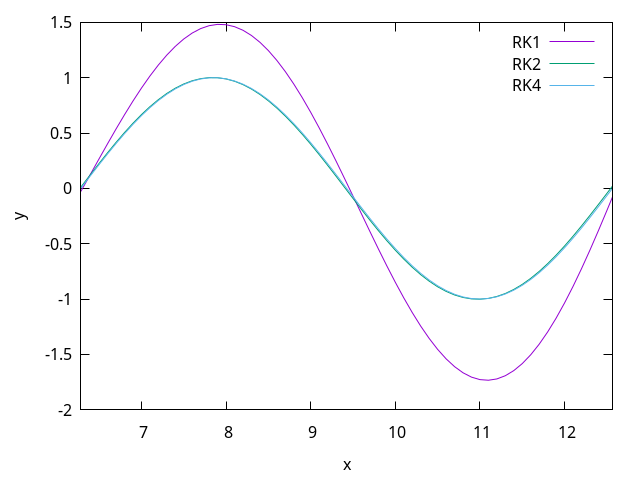
\includegraphics[width=1.5\textwidth]{oscillator_comparison.png}
		      \caption{Confronto tra soluzioni numeriche con step $h=0.1$}
		      \label{fig:sin_comparison}
		      \labfig{expfunc}
	      \end{marginfigure}

	      \begin{marginfigure}
		      \hspace*{-2cm}
		      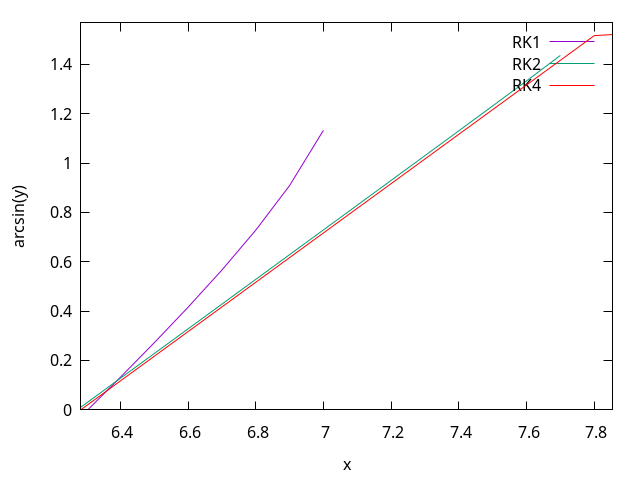
\includegraphics[width=1.5\textwidth]{arcsin_comparison.png}
		      \caption{Visualizzazione alternativa per le soluzioni numeriche
			      (step $h=0.1$)}
		      \label{fig:arcsin_comparison}
		      \labfig{expfunc}
	      \end{marginfigure}

	\item La risoluzione analitica è immediata:
	      \begin{align*}
		      \theta(t) & = Ae^{\lambda t} \rightarrow \lambda^2 + 1 = 0 \\
		      \theta(t) & = Ae^{it} + Be^{-it}                           \\
	      \end{align*}
	      \[
		      \begin{cases}
			      \theta(0) = 0 \\
			      \dot{\theta(0)} = 1
		      \end{cases}
		      \Rightarrow
		      \begin{cases}
			      A+B=0 \\
			      Ai-Bi = 1
		      \end{cases}
		      \Rightarrow
		      \theta(t) = \sin(t)
	      \]

	      Un modo per studiare l'errore è quello di valutare la
	      differenza $\eta(t_{max}, h) - \theta(t_{max})$ (poichè l'effetto di
	      propagazione dell'errore sulla approssimazione è massimo per $t_{max}$). \\
	      Campionando $(e(t_{max}, h_i), h_i)$ si ottiene la figura
	      \ref{fig:error_comparison} si può notare che, come dettato dalla
	      teoria, il metodo RK1 scala come $h$, RK2 come ${h}^2$ e RK4 come $h^{4}$.

	      \begin{marginfigure}
		      \hspace*{-2cm}
		      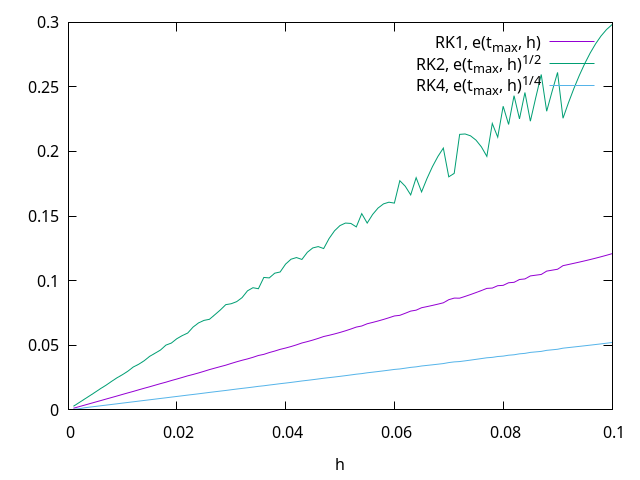
\includegraphics[width=1.5\textwidth]{ode_error_comparison.png}
		      \caption{Associando alla funzione $e(t_{max}, h)$ l'inverso della
			      funzione teoricamente associata si ottiene una relazione di
			      proporzionalità diretta tra le funzioni inverse e $h$}
		      \label{fig:error_comparison}
		      \labfig{expfunc}
	      \end{marginfigure}




	      %TODO: analisi errore, come possiamo valutare e confrontare gli 
	      % ordini?l

	      %% TODO: ulteriori metodi potrebbero essere la media quadratica
\end{enumerate}



\subsection{Oscillatore reale}

\paragraph{Richiesta}

Considerare l'equazione differenziale del pendolo senza l'approssimazione delle piccole oscillazioni:

\begin{equation}
	\ddot{\theta}(t) = -\sin{\theta(t)}
\end{equation}
con $\theta(0) = 0$ e $\dot{\theta}(0) = 1$.

\begin{enumerate}
	\item Risolvere numericamente l'equazione differenziale e tracciare il grafico di $\theta(t)$ e $\dot{\theta}(t)$ e $\dot{\theta}({\theta})$.
	\item Ripetere l'esercizio includendo un termine di attrito:
	      \[
		      \ddot{\theta}(t) = -\sin{\theta(t)} - \gamma \dot{\theta}(t)
	      \]
	\item e un termine forzante:
	      \[
		      \ddot{\theta}(t) = -\sin{\theta(t)} - \gamma \dot{\theta}(t) + A \sin{\frac{2}{3}t}
	      \]
	      con $\gamma \in (0, 2)$ e $A \in (0, 2)$.

\end{enumerate}

\paragraph{Implementazione}

\subparagraph{File necessari} \texttt{damped\_oscillator.cpp}

L'implmentazione necessita solamente di scrivere il sistema di equazioni differenziali, di seguito e' proposta l'implementazione del terzo punto:

\begin{lstlisting} [language=C++]
tensor::Tensor<double> ForcedOscillator(double t,
                                        tensor::Tensor<double> const &y) {
  auto dydt = tensor::Tensor<double>::Vector(2);

  // Dividiamo l'equazione differenziale di secondo ordine 
  // in due di primo ordine
  dydt(0) = y(1);

  // Le costanti vengono passate globalmente
  dydt(1) = -sin(y(0)) - kGamma * y(1) + kA * sin((2.0 / 3) * t);

  return dydt;
}
\end{lstlisting}

\paragraph{Osservazioni e analisi risultati}

\begin{enumerate}

	\item Si ottengono i seguenti risultati per il primo punto, si utilizza inoltre, per limitare i plot ottenuti, che il metodo utilizzato sia \textit{RK4}:

	      \begin{figure} [H]
		      \centering
		      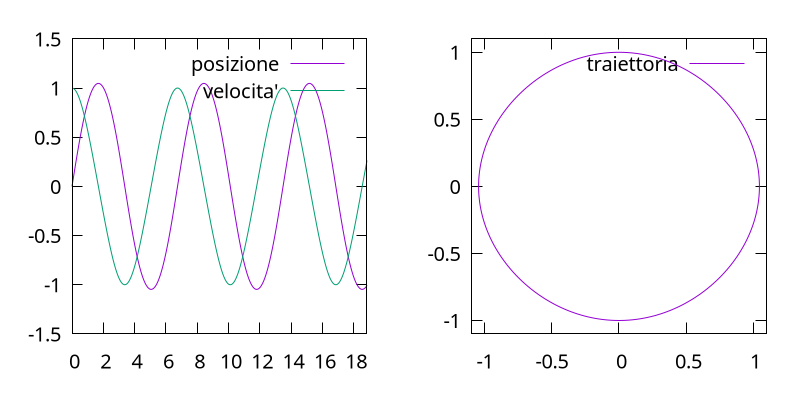
\includegraphics[width=1\textwidth]{real_oscillator_1.png}
		      \caption{Oscillatore ideale imperturbato $(\theta(0)=0, \dot{\theta}(0)=1)$, nel caso di equilibrio stabile. Nella prima figura si possono osservare $\theta(t), \dot{\theta}(t)$, nel secondo $\dot{\theta}(\theta)$, lo spazio delle fasi}
		      \labfig{real_oscil_1}
	      \end{figure}

	      \begin{figure} [H]
		      \centering
		      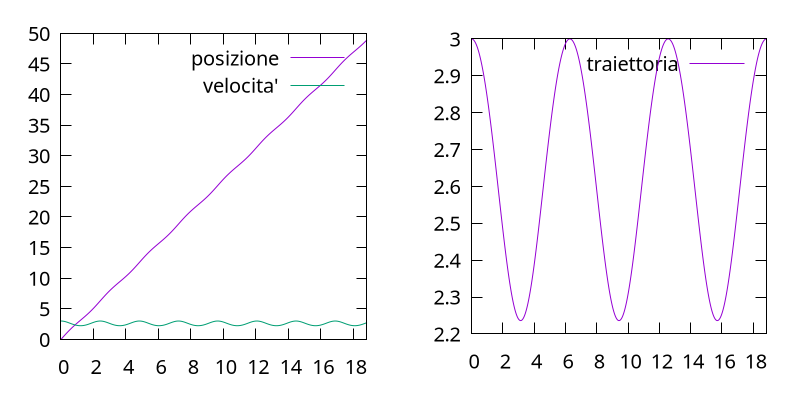
\includegraphics[width=1\textwidth]{real_oscillator_1_1.png}
		      \caption{Oscillatore ideale imperturbato $(\theta(0)=0, \dot{\theta}(0)=3)$, nel caso non in equilibro.}
		      \labfig{real_oscil_1_1}
	      \end{figure}

	      Come si puo' osservare lo spazio delle fasi e' composto principalmente da due
	      casi di traiettorie: la prima in \reffig{real_oscil_1} corrisponde ad un ellisse; mentre, se l'energia cinetica supera l'energia potenziale di carattere oscillatoria, si osserva il caso non in equilibrio: al di sopra e al di sotto delle possibili traiettorie ellissoidali si ottengono traiettorie sinusoidali come in \reffig{real_oscil_1_1}. I risultati corrispondono correttamete con la teoria.

	\item Nel caso dell'oscillatore smorzato si ottengono i seguenti risultati:

	      \begin{figure} [H]
		      \centering
		      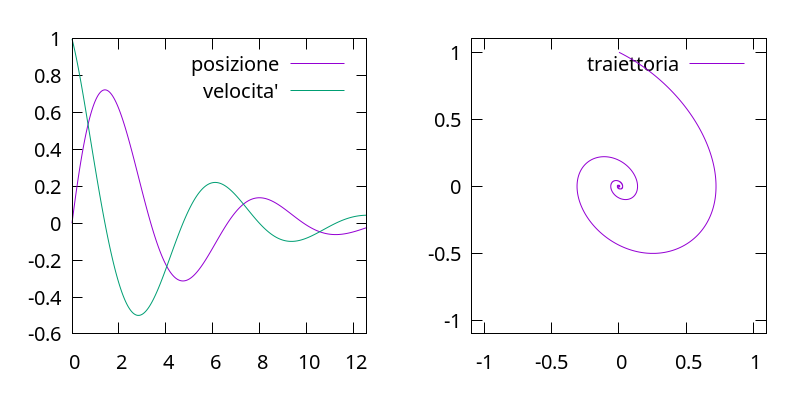
\includegraphics[width=1\textwidth]{real_oscillator_2_0.5.png}
		      \caption{Oscillatore ideale smorzato $(\theta(0)=0, \dot{\theta}(0)=1)$, nel caso $\gamma=0.5$.}
		      \labfig{real_oscil_2_0.5}
	      \end{figure}

	      \begin{figure} [H]
		      \centering
		      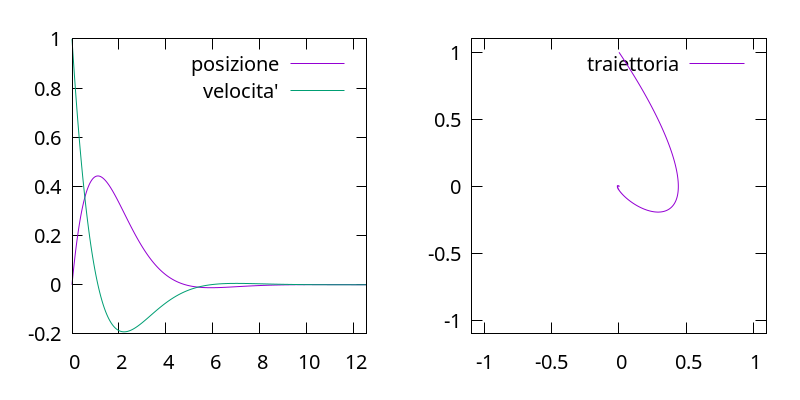
\includegraphics[width=1\textwidth]{real_oscillator_2_1.5.png}
		      \caption{Oscillatore ideale imperturbato $(\theta(0)=0, \dot{\theta}(0)=1)$, nel caso $\gamma=1.5$.}
		      \labfig{real_oscil_2_1.5}
	      \end{figure}

	      Si osserva in questo caso che il termine di smorzamento influenza la traiettoria delle oscillazioni, in particolare, per $\gamma=0.5$ si osserva un'oscillazione smorzata, mentre per $\gamma=1.5$ si osserva un'oscillazione smorzata simil-critica. Lo spazio delle fasi assume una traiettoria a spirale: la spiegazione fisica e' molto semplice, lo smorzamento porta ad un continuo rallentamento del sistema che e' destinato (qualsiasi siano i valori iniziali) a convergere ad un punto. Per questa ragione non vengono inclusi casi di valori iniziali differenti poiche' si otterra' sempre un carattere oscillatorio iniziale per sistemi inizialmente non stabili ma che cadranno necessariamente in una spirale simile alle sovracitate.

	\item Si studia,infine, il caso di smorzamento forzato:

	      \begin{figure} [H]
		      \centering
		      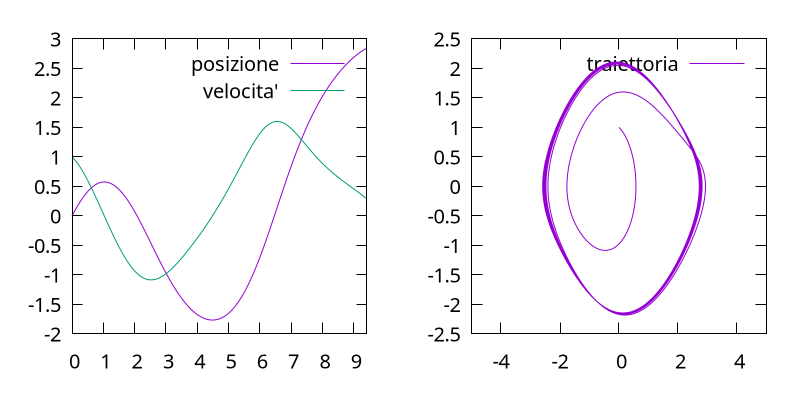
\includegraphics[width=1\textwidth]{real_oscillator_3_0.5_0.5.png}
		      \caption{Oscillatore forzato $(\theta(0)=0, \dot{\theta}(0)=1)$, nel caso $\gamma=0.5, A=0.5$.}
		      \labfig{real_oscil_3_0.5}
	      \end{figure}

	      \begin{figure} [H]
		      \centering
		      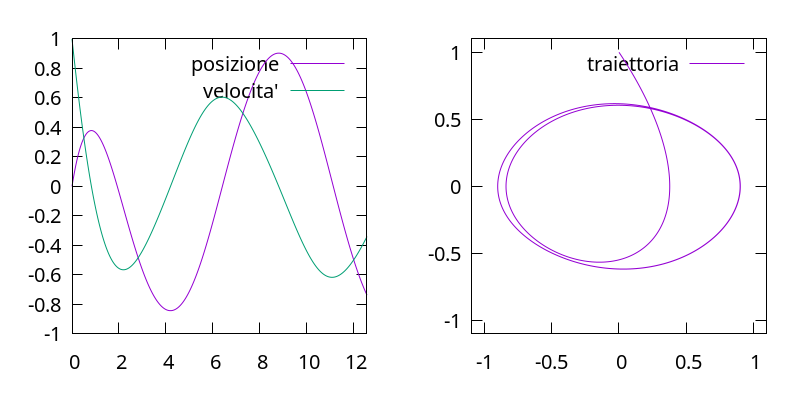
\includegraphics[width=1\textwidth]{real_oscillator_3_1.5_1.5.png}
		      \caption{Oscillatore forzato $(\theta(0)=0, \dot{\theta}(0)=1)$, nel caso $\gamma=1.5, A=1.5$.}
		      \labfig{real_oscil_3_1.5}
	      \end{figure}

	      In \reffig{real_oscil_3_0.5} e in \reffig{real_oscil_3_1.5} si evince chiaramente l'effetto del termine forzante: la traiettoria inizialmente a spirale si dilata e torna ad un caso ellissoide coerentemente con il caso in equilibrio imperturbato. La forzante, il termine $A$, definisce la nuova ampiezza di oscillazione stabile, mentre il termine $\gamma$ definisce la velocità di convergenza al nuovo equilibrio.



\end{enumerate}



\subsection{Attrattore di Lorenz}

\paragraph{Richiesta}

Studiare il sistema di ODE:

\begin{equation}
	\begin{cases}
		\dot{x}(t) = 10(y(t) - x(t))       \\
		\dot{y}(t) = 28x(t) - y(t) - xz(t) \\
		\dot{z}(t) = -8/3 z(t) + xy(t)
	\end{cases}
\end{equation}

\begin{enumerate}
	\item Utilizzare il metodo di Eulero, il metodo di Runge-Kutta del secondo ordine (RK2) e il metodo di Runge-Kutta del quarto ordine (RK4).
	\item Tracciare il grafico di $(x, y)$, $(x, z)$ e $(y, z)$.
\end{enumerate}

\paragraph{Implementazione}

\subparagraph{File necessari} \texttt{lorenz.cpp}

L'implementazione del sistema di equazioni differenziali è immediata essendo gia'
al primo ordine.

\paragraph{Osservazioni e analisi risultati}

Considerando un passo $\Delta t = 0.01$, un intervallo di tempo $t \in [0, 10]$ e valori iniziali $\vec{r}(0)=(0,0,0), \dot{r}(0)=(1,1,1)$ si ottengono le seguenti sezioni della soluzione:

\begin{figure} [H]
	\centering
	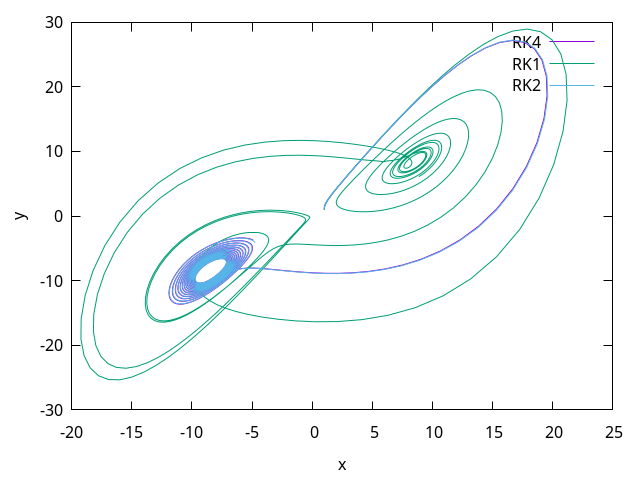
\includegraphics[width=1\textwidth]{lorenz_x_y.png}
	\labfig{real_oscil_3_1.5}
\end{figure}

\begin{figure} [H]
	\centering
	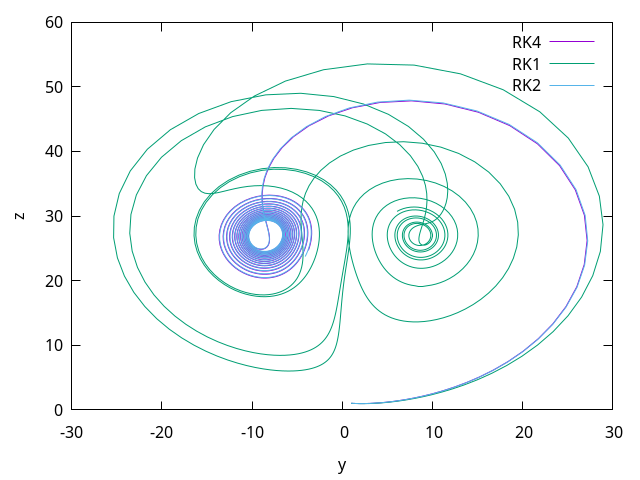
\includegraphics[width=1\textwidth]{lorenz_y_z.png}
	\labfig{real_oscil_3_1.5}
\end{figure}

\begin{figure} [H]
	\centering
	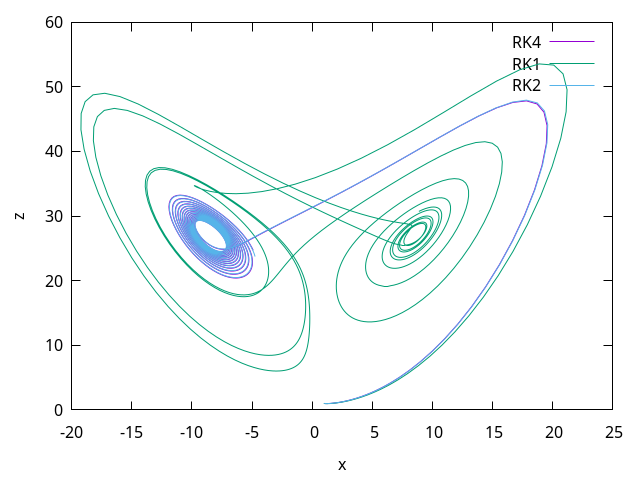
\includegraphics[width=1\textwidth]{lorenz_x_z.png}
	\labfig{real_oscil_3_1.5}
\end{figure}

Il risultato ottenuto e' il noto \textit{Attrattore di Lorenz}, e' inoltre risaputo dalla teoria che il sistema di equazioni differenziali descritto sia caotico: piccole variazioni nei valori iniziali portano a grandi variazioni nel sistema, come si puo' notare dai grafici ottenuti, infatti la differenza dell'ordine del metodo (sopratutto nel metodo di Eulero) porta una variazione considerevole nello step successivo che porta quindi ad un risultato considerevolmente diverso dato un intervallo di tempo adeguato rispetto al differenza tra gli ordine dei metodi considerati. Inoltre, si osserva che il sistema e' invariante per rotazioni, infatti, le traiettorie ottenute sono simmetriche rispetto all'asse $z$.


\subsection{Sistema a tre corpi}

\paragraph{Richiesta}

Studiare il sistema gravitazionale che obbedisce alle equazioni del moto:

\begin{equation}
	\ddot{\vec{x}}_i = \sum_{j \neq i} m_j \; \frac{ \vec{x}_j - \vec{x}_i}{|\vec{x}_j - \vec{x}_i|^3}
	\label{eq:3body}
\end{equation}

Nel caso di tre masse puntiformi, $i = 1, 2, 3$, con i seguenti parametri e condizioni iniziali:

\begin{itemize}
	\item
	      \quad\parbox{\linewidth}{
		      \begin{math}
			      m_1 = m_2 = m_3 = 1 \\
			      \vec{x}_1 = (1, 0, 0), \quad \dot{\vec{x}}_1 = (0, 0.15, -0.15) \\
			      \vec{x}_1 = (-1, 0, 0), \quad \dot{\vec{x}}_1 = (0, -0.15, 0.15) \\
			      \vec{x}_1 = (0, 0, 0), \quad \dot{\vec{x}}_1 = (0, 0, 0)
		      \end{math}
		      \\
	      }
	\item
	      \quad\parbox{\linewidth}{
		      \begin{math}
			      m_1 = 1.6, m_2 = m_3 = 0.4 \\
			      \vec{x}_1 = (1, 0, 0), \quad \dot{\vec{x}}_1 = (0, 0.4, 0) \\
			      \vec{x}_1 = (-1, 0, 0), \quad \dot{\vec{x}}_1 = (0, -0.8, 0.7) \\
			      \vec{x}_1 = (0, 0, 0), \quad \dot{\vec{x}}_1 = (0, -0.8, -0.7)
		      \end{math}
	      }
\end{itemize}

\begin{enumerate}
	\item Risolvere numericamente il sistema di equazioni.
	\item Tracciare il grafico dell'energia totale del sistema in funzione del tempo.
\end{enumerate}

\paragraph{Implementazione}

\subparagraph{File necessari} \texttt{gravitation.cpp}

Nella matrice della soluzione si sceglie di ordinare la soluzione ad ogni time step nel seguente modo:

\[
	\begin{pmatrix}
		r_{1,x}(t_0) & r_{1,y}(t_0) & \dots & r_{3,z}(t_0) & v_{1,x}(t_0) & \dots & v_{3,z}(t_0) \\
		\vdots                                                                                   \\

		r_{1,x}(t_n) & r_{1,y}(t_n) & \dots & r_{3,z}(t_n) & v_{1,x}(t_n) & \dots & v_{3,z}(t_n) \\
	\end{pmatrix}
\]

La funzione che definisce il sistema dovra' quindi tradurre l'equazione \ref{eq:3body} in un sistema di equazioni differenziali al primo ordine che rispettino l'ordine della matrice:

\begin{lstlisting} [language=C++]
...
  // Calcoliamo la accelerazione di interazione per ogni corpo
  auto grav_accell = [&](int i, int j) -> tensor::Tensor<double> {
    auto r_ij = tensor::Tensor<double>::Vector(3);
    for (int k = 0; k < 3; k++) {
      // Utilizziamo l'ordine specificato nella matrice
      r_ij(k) = y(3 * i + k) - y(3 * j + k);
    }

    double dist = r_ij.Norm();
    double dist_cubed = std::pow(dist, 3);

    auto accell = tensor::Tensor<double>::Vector(3);

    for (int k = 0; k < 3; ++k) {
      accell(k) = -masses(j) * r_ij(k) / dist_cubed;
    }

    return accell;
  };

  for (int i = 0; i < 3; ++i) {
    for (int k = 0; k < 3; ++k) {
      // Vengono aggiornate le posizioni
      dydt(3 * i + k) = y(3 * (i + 3) + k);
    }

    auto acc = tensor::Tensor<double>::Vector(3);
    // Utilizzando modulo 3 si riottengono gli indici delle posizioni 
    // dei corpi e calcoliamo l'accelerazione
    auto acc1 = grav_accell(i, (i + 1) % 3);
    auto acc2 = grav_accell(i, (i + 2) % 3);

    for (int k = 0; k < 3; ++k) {
      // Si aggiornano le velocita'
      dydt(3 * (i + 3) + k) = (acc1 + acc2)(k);
    }
  }
\end{lstlisting}

Si ottiene dunque la nuova riga della matrice dal vettore riga \texttt{dydt} allo step successivo.



\paragraph{Osservazioni e analisi risultati}

Utilizzando il metodo $RK4$ e step $\Delta t = 0.01$ si ottengono i seguenti risultati:

\begin{enumerate}
	\item
	      \begin{marginfigure}
		      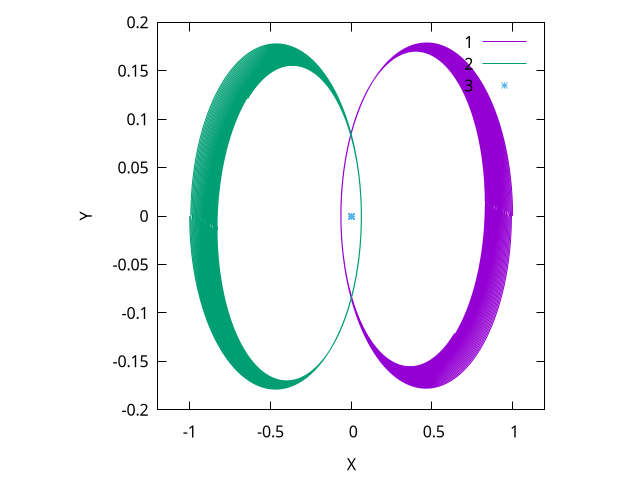
\includegraphics[width=1.5\textwidth]{gravitation_1_xy.png}
		      \caption{Sezione sul piano XY del primo punto}
		      \labfig{grav_1}
	      \end{marginfigure}

	      \begin{marginfigure}
		      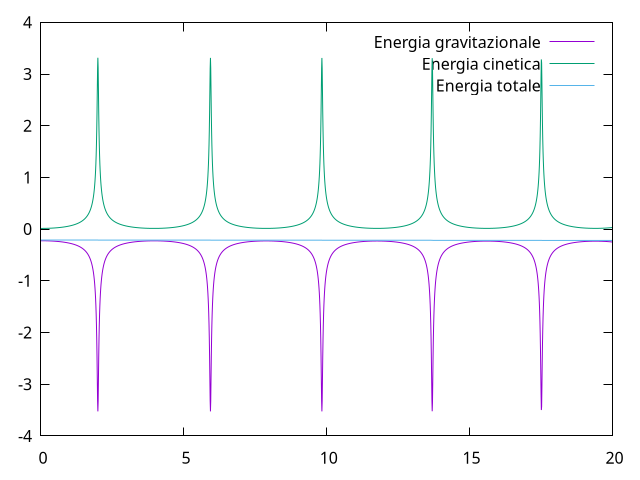
\includegraphics[width=1.5\textwidth]{grav_energy_1.png}
		      \caption{Grafico delle energie per il punto 1}
		      \labfig{grav_energy_1}
	      \end{marginfigure}

	      Dalle figure \reffig{grav_1} e \reffig{grav_energy_1} si osserva che, data la simmetria dei dati iniziali, la traiettoria dei corpi e' simmetrica rispetto all'asse $x$. Inoltre, si osserva che l'energia totale del sistema e' conservata, come ci si aspetta dal sistema gravitazionale, per valori non troppo grandi di $t$, piu' aumenta il tempo piu' il trend dell'energia totale diminuisce seguendo una retta di pendenza negativa, l'approssimazione del metodo $RK4$ dissipa energia per valori grandi di $t$; si conferma, inoltre, la presenza di un sistema legato data la presenza di una energia totale negativa.


	\item
	      \begin{marginfigure}
		      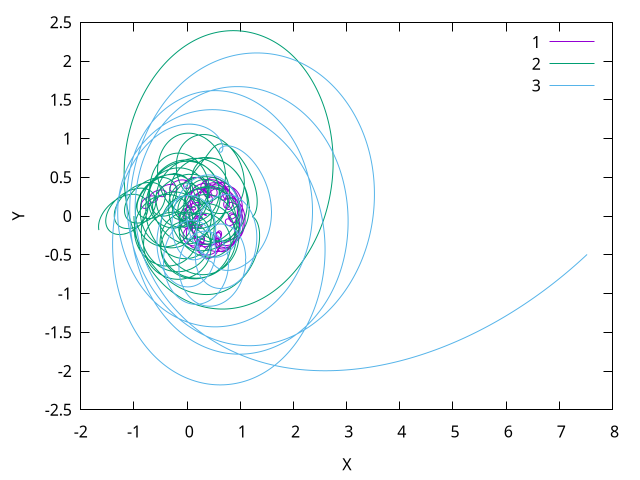
\includegraphics[width=1.5\textwidth]{gravitation_2_xy.png}
		      \caption{Sezione sul piano XY del primo punto}
		      \labfig{grav_2}
	      \end{marginfigure}

	      \begin{marginfigure}
		      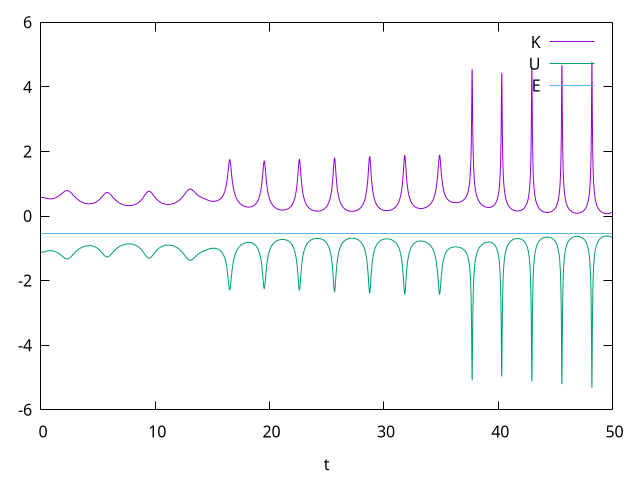
\includegraphics[width=1.5\textwidth]{grav_energy_2.png}
		      \caption{Grafico delle energie per il punto 2}
		      \labfig{grav_energy_2}
	      \end{marginfigure}

	      % Stesso trend negativo per le energie, il sistema e' in questo caso instabile 

        Nei grafici \reffig{grav_2} e \reffig{grav_energy_2} si osserva che il sistema e' caotico e legato. Si ripresenta nuovamente la pendenza negativa dell'energia totale seppure con un coefficiente relativamente basso non apprezabile a queste scale.


\paragraph{Conclusioni}

I metodi Runge-Kutta utilizzati negli esercizi non garantiscono la conservazione dell'energia del sistema: quando i corpi si avvicinano molto tra di loro si perdono molte informazioni sul sistema, quest'ultime e l'intervallo di step utilizzato non sono adeguatamente distribuiti rispetto alla forza esercitata tra i due corpi nello step corrente. Utilizzando degli intervalli di tempo in funzione della distanza tra i corpi si otterrebbero misure piu' precise, utilizzando, come nel seguente esercizio, uno step fisso nel calcolo si perdono informazioni quando i corpi sono piu' vicini e quindi molto piu' veloci. Oltre a questa soluzione personalmente ipotizzata si possono utilizzare metodi che garantiscono la conservazione di dell'energia: i \textit{Metodi Simplettici} 

%TODO: citare metodi simplettici







\end{enumerate}











\setchapterpreamble[u]{\margintoc}
\chapter{Equazione di Schrödinger}
\labch{schroedinger}

\section{Esercizi}

\subsection{Esercizio 16}

\paragraph{Nozioni teoriche}

%TODO: scrivere nozioni teoriche

Si ottiene dunque, nel caso particolare del problema:

\[
	\left[-\frac{N^2}{16}K+\mathcal{V}\right]\phi = \mathcal{E} \phi \quad \mathcal{E} = EL, \mathcal{V} = VL
\]

con $K_{ii} = -2, K_{j+1,j}=K_{j,j+1}=1 \quad 0 \leq j < N-1, \; 0 \leq i < N$. \\$V= -V_0$ per $1/4 \leq x \leq 3/4$


\paragraph{Implementazione}

\label{file}
\subparagraph{File necessari} \texttt{ex\_16.cpp}

L'implementazione segue direttamente dalla equazione sopracitata applicando il \textit{Power Deflation Method}

\paragraph{Analisi dei risultati e conclusioni}

\begin{enumerate}

	\item Si veda \texttt{ex\_16.cpp}

	\item

	      \begin{marginfigure}
		      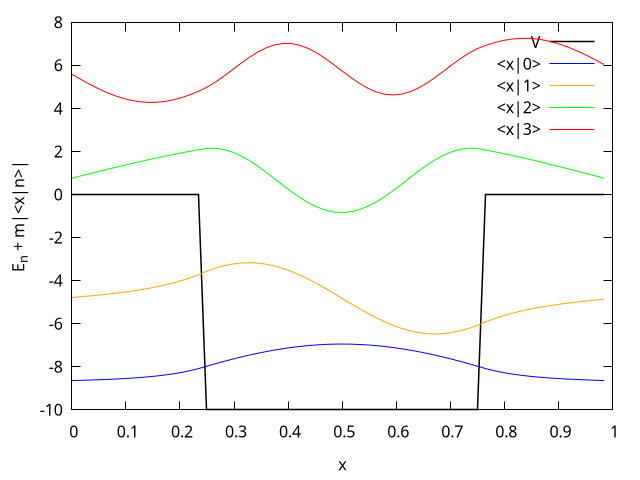
\includegraphics[width=1.5\textwidth]{schroedinger_1_1.png}
		      \caption{Autofunzioni della buca finita di potenziale}
		      \label{fig:schroedinger_1_1}
	      \end{marginfigure}

	      Come ci si aspetta si ottengono stati legati che qualitativamente possono essere considerati corretti: i nodi corrispondono all'energia dello stato; all'interno della parete la funzione d'onda scala come un'esponenziale; nei casi al di sopra della parete si ottengono oscillazioni a frequenza piu' alta per $E-V$ piu' grandi.


	\item
	      \begin{marginfigure}
		      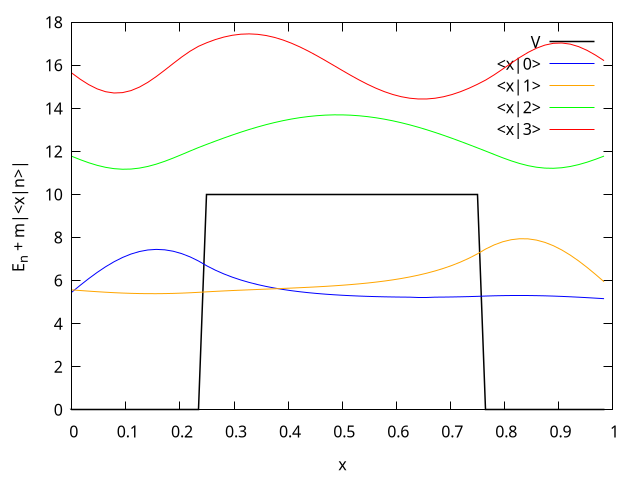
\includegraphics[width=1.5\textwidth]{schroedinger_1_2.png}
		      \caption{Autofunzioni della buca finita di potenziale}
		      \label{fig:schroedinger_1_2}
	      \end{marginfigure}
	\item


	      \begin{marginfigure}
		      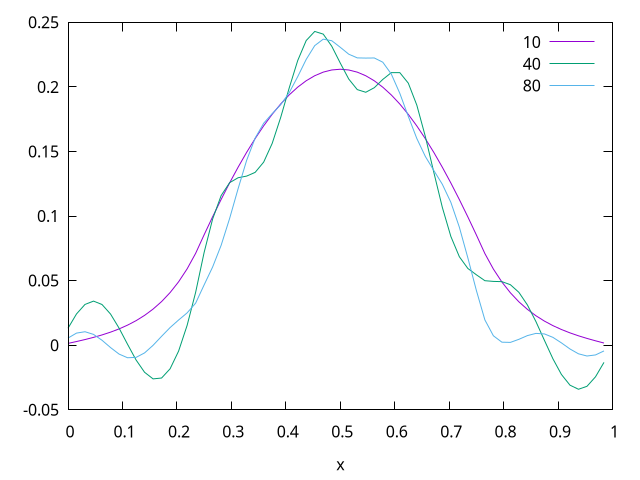
\includegraphics[width=1.5\textwidth]{schroedinger_1_3.png}
		      \caption{Autofunzioni della buca finita di potenziale}
		      \label{fig:schroedinger_1_3}
	      \end{marginfigure}
	\item


	      \begin{marginfigure}
		      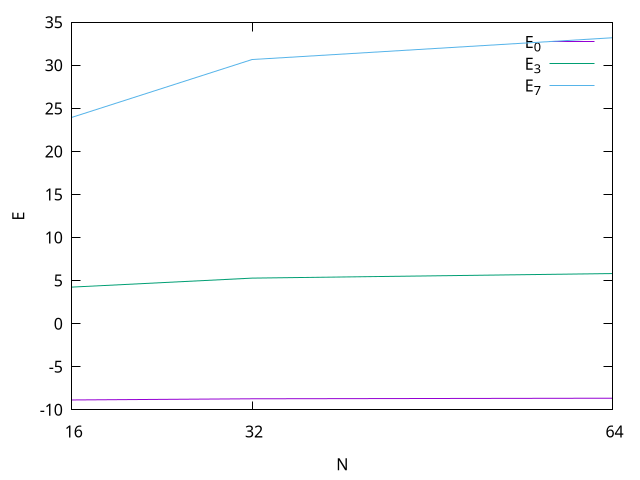
\includegraphics[width=1.5\textwidth]{schroedinger_1_4.png}
		      \caption{Autofunzioni della buca finita di potenziale}
		      \label{fig:schroedinger_1_4}
	      \end{marginfigure}

\end{enumerate}

\subsection{Esercizio 17}

\paragraph{Nozioni teoriche}

\paragraph{Implementazione}

\paragraph{Analisi dei risultati e conclusioni}








\setchapterpreamble[u]{\margintoc}
\chapter{Metodi di integrazione}
\labch{integration}




\iffalse
\setchapterpreamble[u]{\margintoc}
\chapter{Margin Stuff}

Sidenotes are a distinctive feature of all 1.5-column-layout books. 
Indeed, having wide margins means that some material can be displayed 
there. We use margins for all kind of stuff: sidenotes, marginnotes, 
small tables of contents, citations, and, why not?, special boxes and 
environments.

\section{Sidenotes}

Sidenotes are like footnotes, except that they go in the margin, where 
they are more readable. To insert a sidenote, just use the command 
\Command{sidenote\{Text of the note\}}. You can specify a 
mark\sidenote[O]{This sidenote has a special mark, a big O!} with \\ 
\Command{sidenote[mark]\{Text\}}, but you can also specify an offset, 
which moves the sidenote upwards or downwards, so that the full syntax is:

\begin{lstlisting}[style=kaolstplain]
\sidenote[mark][offset]{Text}
\end{lstlisting}

If you use an offset, you always have to add the brackets for the mark, 
but they can be empty.\sidenote{If you want to know more about the usage 
of the \Command{sidenote} command, read the documentation of the 
\Package{sidenotes} package.}

In \Class{kaobook} we copied a feature from the \Package{snotez} 
package: the possibility to specify a multiple of \Command{baselineskip} 
as an offset. For example, if you want to enter a sidenote with the 
normal mark and move it upwards one line, type:

\begin{lstlisting}[style=kaolstplain]
\sidenote[][*-1]{Text of the sidenote.}
\end{lstlisting}

As we said, sidenotes are handled through the \Package{sidenotes} 
package, which in turn relies on the \Package{marginnote} package.

\section{Marginnotes}

This command is very similar to the previous one. You can create a 
marginnote with \Command{marginnote[offset]\{Text\}}, where the offset 
argument can be left out, or it can be a multiple of 
\Command{baselineskip},\marginnote[-1cm]{While the command for margin 
notes comes from the \Package{marginnote} package, it has been redefined 
in order to change the position of the optional offset argument, which 
now precedes the text of the note, whereas in the original version it 
was at the end. We have also added the possibility to use a multiple of 
\Command{baselineskip} as offset. These things were made only to make 
everything more consistent, so that you have to remember less things!} 
\eg

\begin{lstlisting}[style=kaolstplain]
\marginnote[-12pt]{Text} or \marginnote[*-3]{Text}
\end{lstlisting}

\begin{kaobox}[frametitle=To Do]
A small thing that needs to be done is to renew the \Command{sidenote} 
command so that it takes only one optional argument, the offset. The 
special mark argument can go somewhere else. In other words, we want the 
syntax of \Command{sidenote} to resemble that of \Command{marginnote}.
\end{kaobox}

We load the packages \Package{marginnote}, \Package{marginfix} and 
\Package{placeins}. Since \Package{sidenotes} uses \Package{marginnote}, 
what we said for marginnotes is also valid for sidenotes. Side- and 
margin- notes are shifted slightly upwards 
(\Command{renewcommand\{\textbackslash marginnotevadjust\}\{3pt\}}) in 
order to align them to the bottom of the line of text where the note is 
issued. Importantly, both sidenotes and marginnotes are defined as 
floating if the optional argument (\ie the vertical offset) is left 
blank, but if the offset is specified they are not floating. Recall that 
floats cannot be nested, so in some rare cases you may encounter errors 
about lost floats; in those cases, remember that sidenotes and 
marginnotes are floats. To solve the problem, it may be possible to 
transform them into non-floating elements by specifying an offset of 
0pt.

\section{Footnotes}

Even though they are not displayed in the margin, we will discuss about 
footnotes here, since sidenotes are mainly intended to be a replacement 
of them. Footnotes force the reader to constantly move from one area of 
the page to the other. Arguably, marginnotes solve this issue, so you 
should not use footnotes. Nevertheless, for completeness, we have left 
the standard command \Command{footnote}, just in case you want to put a 
footnote once in a while.\footnote{And this is how they look like. 
Notice that in the PDF file there is a back reference to the text; 
pretty cool, uh?}

\section{Margintoc}

Since we are talking about margins, we introduce here the 
\Command{margintoc} command, which allows one to put small table of 
contents in the margin. Like other commands we have discussed, 
\Command{margintoc} accepts a parameter for the vertical offset, like 
so: \Command{margintoc[offset]}.

The command can be used in any point of the document, but we think it 
makes sense to use it just at the beginning of chapters or parts. In 
this document I make use of a \KOMAScript\xspace feature and put it in 
the chapter preamble, with the following code:

\marginnote{The font used in the margintoc is the same as the one for 
	the chapter entries in the main table of contents at the beginning 
	of the document.}

\begin{lstlisting}[style=kaolstplain]
\setchapterpreamble[u]{\margintoc}
\chapter{Chapter title}
\end{lstlisting}

As the space in the margin is a valuable resource, there is the 
possibility to print a shorter version of the title in the margin toc. 
Thus, there are in total three possible versions for the title of a 
section (or subsection): the one for the main text, the one for the main 
table of contents, and the one for the margintoc. These versions can be 
specified at the same time when the section is created in the source 
\TeX file:
\begin{lstlisting}[style=kaolstplain]
\section[alternative-title-for-toc]{title-as-written-in-text}[alternative-title-for-margintoc]
\end{lstlisting}

By default, the margintoc includes sections and subsections.
If you only want to show sections, add
\begin{lstlisting}[style=kaolstplain]
\setcounter{margintocdepth}{\sectiontocdepth}
\end{lstlisting}
somewhere in your preamble.

\section{Marginlisting}

On some occasions it may happen that you have a very short piece of code 
that doesn't look good in the body of the text because it breaks the 
flow of narration: for that occasions, you can use a 
\Environment{marginlisting}. The support for this feature is still 
limited, especially for the captions, but you can try the following 
code:

\begin{marginlisting}[-1.35cm]
	\caption{An example of a margin listing.}
	\vspace{0.6cm}
	\begin{lstlisting}[language=Python,style=kaolstplain]
print("Hello World!")
	\end{lstlisting}
\end{marginlisting}

\begin{verbatim}
\begin{marginlisting}[-0.5cm]
	\caption{My caption}
	\vspace{0.2cm}
	\begin{lstlisting}[language=Python,style=kaolstplain]
	... code ...
	\end{lstlisting}
\end{marginlisting}
\end{verbatim}

Unfortunately, the space between the caption and the listing must be 
adjusted manually; if you find a better way, please let me know.

Not only textual stuff can be displayed in the margin, but also figures. 
Those will be the focus of the next chapter.

\setchapterimage[7.5cm]{seaside}
\setchapterpreamble[u]{\margintoc}
%\chapter[Figures and Tables]{Figures and Tables\footnotemark[0]}
\chapter{Figures and Tables}

\footnotetext{The credits for the image above the chapter title go to:
	Bushra Feroz, CC~BY-SA~4.0, \url{https://commons.wikimedia.org/w/index.php?curid=68724647}}

\section{Normal Figures and Tables}

Figures and tables can be inserted just like in any standard 
\LaTeX\xspace document. The \Package{graphicx} package is already loaded 
and configured in such a way that the figure width is equal to the 
textwidth and the height is adjusted in order to maintain the original 
aspect ratio. As you may have imagined, the captions will be 
positioned\ldots well, in the margins. This is achieved with the help of 
the \Package{floatrow} package.

Here is a picture of Mona Lisa (\reffig{normalmonalisa}), as an example. 
The captions are formatted as the margin- and the side-notes; If you 
want to change something about captions you can use the command 
\Command{captsetup} from the \Package{caption} package. Remember that if 
you want to reference a figure, the label must come \emph{after} the 
caption!

\begin{figure}[hb]
	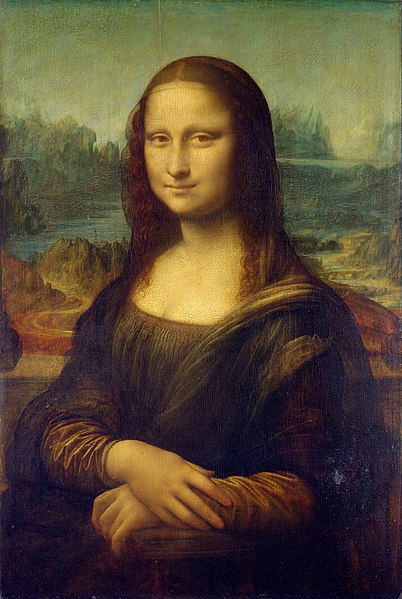
\includegraphics[width=0.45\textwidth]{monalisa}
	\caption[Mona Lisa, again]{It's Mona Lisa again. \blindtext}
	\labfig{normalmonalisa}
\end{figure}

While the format of the caption is managed by \Package{caption}, its 
position is handled by the \Package{floatrow} package. Achieving this 
result has been quite hard, but now I am pretty satisfied. In two-side 
mode, the captions are printed in the correct margin.

Tables can be inserted just as easily as figures, as exemplified by the 
following code:

\begin{lstlisting}[caption={Caption of a listing.}]
\begin{table}
\begin{tabular}{ c c c c }
	\toprule
	col1 & col2 & col3 & col 4 \\
	\midrule
	\multirow{3}{4em}{Multiple row} & cell2 & cell3 & cell4\\ &
	cell5 & cell6 & cell7 \\ &
	cell8 & cell9 & cell10 \\
	\multirow{3}{4em}{Multiple row} & cell2 & cell3 & cell4 \\ &
	cell5 & cell6 & cell7 \\ &
	cell8 & cell9 & cell10 \\
	\bottomrule
\end{tabular}
\end{table}
\end{lstlisting}

which results in the useless \vreftab{useless}.

\begin{table}[ht]
\caption[A useless table]{A useless table.}
\labtab{useless}
\begin{tabular}{ c c c c }
	\toprule
	col1 & col2 & col3 & col 4 \\
	\midrule
	\multirow{3}{4em}{Multiple row} & cell2 & cell3 & cell4\\ &
	cell5 & cell6 & cell7 \\ &
	cell8 & cell9 & cell10 \\
	\multirow{3}{4em}{Multiple row} & cell2 & cell3 & cell4 \\ &
	cell5 & cell6 & cell7 \\ &
	cell8 & cell9 & cell10 \\
	\bottomrule
\end{tabular}
\end{table}

I don't have much else to say, so I will just insert some blind text. 
\blindtext

\section{Margin Figures and Tables}

Marginfigures can be inserted with the environment 
\Environment{marginfigure}. In this case, the whole picture is confined 
to the margin and the caption is below it. \reffig{marginmonalisa} is 
obtained with something like this:

\begin{lstlisting}[caption={Another caption.}]
\begin{marginfigure}
	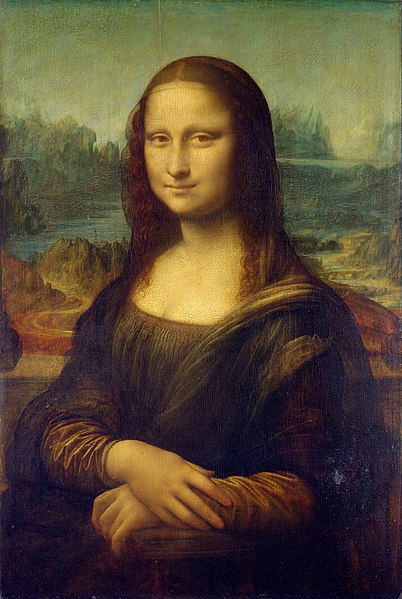
\includegraphics{monalisa}
	\caption[The Mona Lisa]{The Mona Lisa.}
	\labfig{marginmonalisa}
\end{marginfigure}
\end{lstlisting}

There is also the \Environment{margintable} environment, of which 
\reftab{anotheruseless} is an example. Notice how you can place the 
caption above the table by just placing the \Command{caption} command 
before beginning the \Environment{tabular} environment. Usually, figure 
captions are below, while table captions are above. This rule is also 
respected for normal figures and tables: the captions are always on the 
side, but for figure they are aligned to the bottom, while for tables to 
the top.

\begin{margintable}
\caption[Another useless table]{Another useless table.}
\labtab{anotheruseless}
\raggedright
\begin{tabular}{ c c c c }
	\hline
	col1 & col2 & col3 \\
	\hline
	\multirow{3}{4em}{Multiple row} & cell2 & cell3 \\ & cell5 & cell6 
	\\ & cell8 & cell9 \\ \hline
\end{tabular}
\end{margintable}

Marginfigures and tables can be positioned with an optional offset 
command, like so:

\begin{lstlisting}
\begin{marginfigure}[offset]
	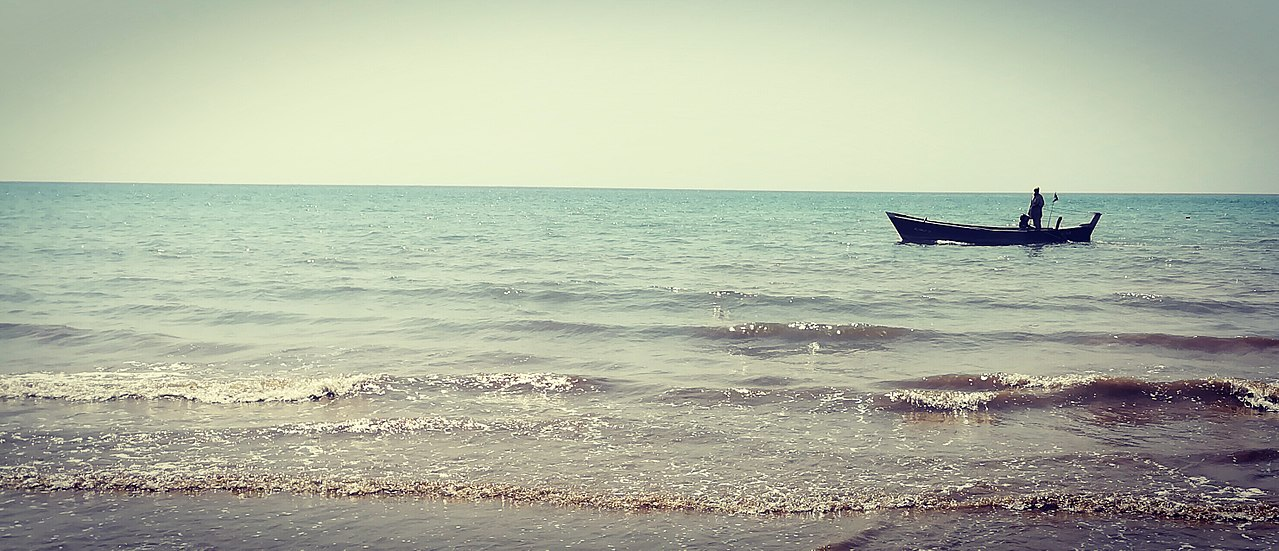
\includegraphics{seaside}
\end{marginfigure}
\end{lstlisting}

Offset ca be either a measure or a multiple of \Command{baselineskip}, 
much like with \Command{sidenote}, \Command{marginnote} and 
\Command{margintoc}.\todo{Improve this part.} If you are wondering how I 
inserted this orange bubble, have a look at the \Package{todo} package.

\section{Wide Figures and Tables}

With the environments \Environment{figure*} and \Environment{table*} you 
can insert figures which span the whole page width. For example, here 
are a wide figure and a wide table.

\begin{figure*}[h!]
	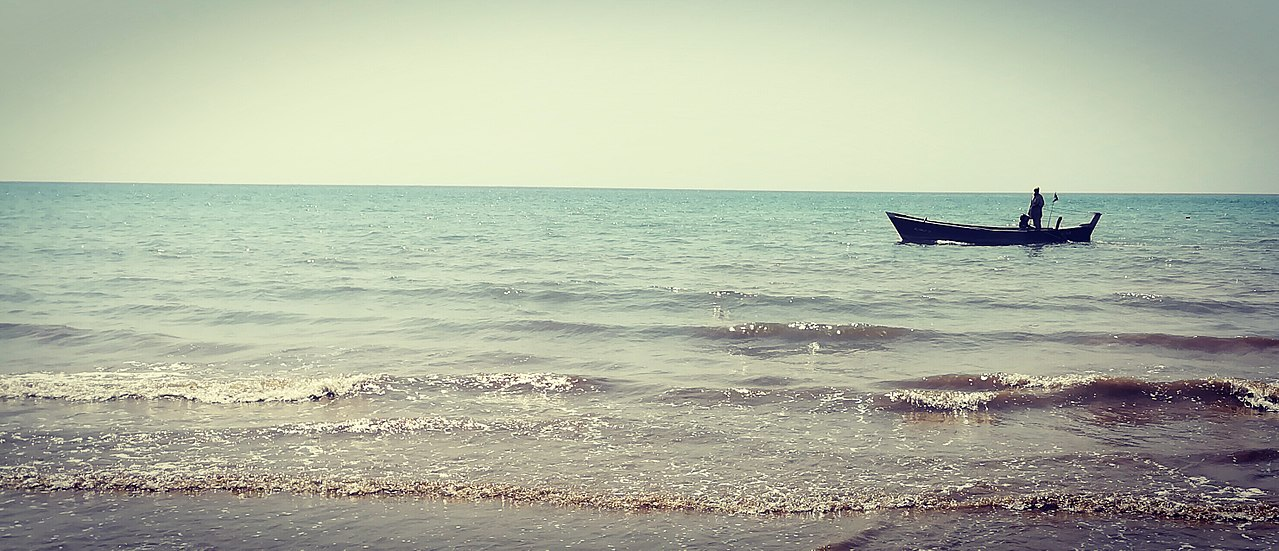
\includegraphics{seaside}
	\caption[A wide seaside]{A wide seaside, and a wide caption.
		Credits: By Bushra Feroz, CC BY-SA 4.0, \url{https://commons.wikimedia.org/w/index.php?curid=68724647}}
\end{figure*}

\begin{table*}[h!]
    \caption{A wide table with invented data about three people living in the UK. Note that wide figures and tables are centered and their caption also extends into the margin.}
    \begin{tabular}{p{2.0cm} p{2.0cm} p{2.0cm} p{2.0cm} p{2.0cm} p{2.0cm} p{1.5cm}}
        \toprule
        Name    & Surname   & Job       & Salary           & Age   & Height    & Country \\
        \midrule
        Alice   & Red       & Writer    & 4.000 \pounds    & 34    & 167 cm     & England \\
        Bob     & White     & Bartender & 2.000 \pounds    & 24    & 180 cm     & Scotland \\
        Drake   & Green     & Scientist & 4.000 \pounds    & 26    & 175 cm     & Wales \\
        \bottomrule
    \end{tabular}
\end{table*}

It is the user's responsibility to adjust the width of the table, if 
necessary, until it is aesthetically pleasing. The previous table was 
obtained with the following code:

\begin{lstlisting}[caption=How to typeset a wide table]
\begin{table*}[h!]
    \caption{A wide table with invented data about three people living in the UK. Note that wide figures and tables are centered and their caption also extends into the margin.}
    \begin{tabular}{p{2.0cm} p{2.0cm} p{2.0cm} p{2.0cm} p{2.0cm} p{2.0cm} p{1.5cm}}
        \toprule
        Name    & Surname   & Job       & Salary           & Age   & Height    & Country \\
        \midrule
        Alice   & Red       & Writer    & 4.000 \pounds    & 34    & 167 cm     & England \\
        Bob     & White     & Bartender & 2.000 \pounds    & 24    & 180 cm     & Scotland \\
        Drake   & Green     & Scientist & 4.000 \pounds    & 26    & 175 cm     & Wales \\
        \bottomrule
    \end{tabular}
\end{table*}
\end{lstlisting}

The \Package{floatrow} package provides the \enquote{H} specifier to 
instruct \LaTeX to position the figure (or table) in precisely the same 
position it occupies in the source code. However, this specifier does 
not work with wide figures or tables: you should use \enquote{h!} 
instead, like so: \lstinline|\begin{figure*}[h!]|.

You may have noticed the full width image at the very beginning of this
chapter: that, however, is set up in an entirely different way, which
you'll read about in \vrefch{layout}.

\Class{kaobook} also supports paginated tables (have a look at the 
\Package{longtable} package). The 
\Environment{longtable}\sidenote{Interestingly, \Environment{longtable}s 
may require up to four rounds of compilation before they are typeset 
correctly.} environment behaves a bit differently from 
\Environment{table}, in that \Environment{longtable} encompasses both 
\Environment{table} and \Environment{tabular}, so that you can write, 
\eg,

\begin{lstlisting}[caption=Example of a longtable]
\begin{longtable}{|l c c|}
    \hline
    One & Two & Three \\
    Left & Center & Center \\
    \hline
    \caption{Caption of the longtable.}
\end{longtable}
\end{lstlisting}

to obtain the following table:
\begin{longtable}{|l c c|}
    \hline
    One & Two & Three \\
    Left & Center & Center \\
    \hline
    \caption{Caption of the longtable.}
\end{longtable}

The caption of a \Environment{longtable} is always positioned below the 
table, and it has the same width as the text (it doesn't extend into the 
margin). However, sometimes you may need a \Environment{longtable} that 
is so wide that it trespass into the margins; in those cases, you may 
want to also increase the width of the caption. To do so, you'll have to 
write two additional commands, one before and one after the 
\Environment{longtable}:

\begin{lstlisting}[caption=Increasing the width of the caption of a \Environment{longtable}.]
\floatsetup[longtable]{margins=centering,LTcapwidth=table} % Add this line before the longtable to increase the caption width
\begin{longtable}{lp{8cm}p{5cm}p{2cm}}
...
\end{longtable}
\floatsetup[longtable]{margins=raggedright,LTcapwidth=\textwidth} % Add this line after the longtable to revert the previous change
\end{lstlisting}

Having seen figures and tables, it is now time to tackle 
hyperreferences.

\setchapterstyle{kao}
%\setchapterpreamble[u]{\margintoc}
\chapter{References}
\labch{references}

\section{Citations}

\index{citations}
To cite someone \sidecite{Visscher2008,James2013} is very simple: just 
use the \Command{sidecite}\index{\Command{sidecite}} command. It does 
not have an offset argument yet, but it probably will in the future. 
This command supports multiple entries, as you can see, and by default 
it prints the reference on the margin as well as adding it to the 
bibliography at the end of the document. Note that the citations have 
nothing to do with the text,\sidecite{James2013} but they are completely 
random as they only serve the purpose to illustrate the feature.

For this setup I wrote a separate package, \Package{kaobiblio}, which 
you can find in the \Package{styles} directory and include in your main 
tex file. This package accepts all the options that you can pass to 
\Package{biblatex}, and actually it passes them to \Package{biblatex} 
under the hood. Moreover, it also defines some commands, like 
\Command{sidecite}, and environments that can be used within a 
\Class{kao} book.\sidenote[][-.9cm]{For this reason you should always 
use \Package{kaobiblio} instead of \Package{biblatex}, but the syntax 
and the options are exactly the same.}

If you want to use \Package{bibtex} instead of \Package{biblatex},
pass the option \Option{backend=bibtex} to \Package{kaobiblio}.
\Package{kaobiblio} also supports two options that are not shared with
\Package{biblatex}: \Option{addspace} and \Option{linkeverything},
both of which are boolean options, meaning that they can take
either \enquote{true} or \enquote{false} as a value. If you
pass \Option{addspace=true} when loading \Package{kaobiblio},
a space will be automatically added before the citation marks.
If you pass \Option{linkeverything=true}, the author's name in
the authoryear-* and authortitle-* styles will be a hyperlink
like the year.\sidenote{The fact that the author name is not
a hyperlink bothers more than one biblatex user. There are
\href{https://github.com/plk/biblatex/issues/428}{strong arguments}
\emph{against} hyperlinking the author name, but in my personal opinion, 
linking the author's name does not result in any problems in most 
practical cases.}

As you have seen, the \Command{sidecite} command will print a citation 
in the margin. However, this command would be useless without a way to 
customise the format of the citation, so the \Class{kaobook} provides 
also the \Command{formatmargincitation} command. By \enquote{renewing} 
that command, you can choose which items will be printed in the margins. 
The best way to understand how it works is to see the actual definition 
of this command.

\begin{lstlisting}[style=kaolstplain,linewidth=1.5\textwidth]
\newcommand{\formatmargincitation}[1]{%
	\parencite{#1}: \citeauthor*{#1} (\citeyear{#1}), \citetitle{#1}%
}
\end{lstlisting}

Thus, the \Command{formatmargincitation} accepts one parameter, which is 
the citation key, and prints the parencite followed by a colon, then the 
author, then the year (in brackets), and finally the 
title.\sidecite{Battle2014} Now, suppose that you wish the margin 
citation to display the year and the author, followed by the title, and 
finally a fixed arbitrary string; you would add to your document:

\begin{lstlisting}[style=kaolstplain,linewidth=1.5\textwidth]
\renewcommand{\formatmargincitation}[1]{%
	\citeyear{#1}, \citeauthor*{#1}: \citetitle{#1}; very interesting!%
}
\end{lstlisting}

\renewcommand{\formatmargincitation}[1]{%
	\citeyear{#1}, \citeauthor*{#1}: \citetitle{#1}; very interesting!%
}

The above code results in citations that look like the 
following.\sidecite{Zou2005} Of course, changing the format is most 
useful when you also change the default bibliography style. For 
instance, if you want to use the \enquote{philosophy-modern} style for 
your bibliography, you might have something like this in the preamble:

\begin{lstlisting}[style=kaolstplain,linewidth=1.5\textwidth]
\usepackage[style=philosophy-modern]{styles/kaobiblio}
\renewcommand{\formatmargincitation}[1]{%
	\sdcite{#1}%
}
\addbibresource{main.bib}
\end{lstlisting}

\renewcommand{\formatmargincitation}[1]{%
	\parencite{#1}: \citeauthor*{#1} (\citeyear{#1}), \citetitle{#1}%
}

The commands like \Command{citeyear}, \Command{parencite}
and \Command{sdcite} are just examples. A full
reference of the available commands can be found in this
\href{http://tug.ctan.org/info/biblatex-cheatsheet/biblatex-cheatsheet.pdf}{cheatsheet},
under the \enquote{Citations} section.

Finally, to compile a document containing citations, you need to use an 
external tool, which for this class is biber. You need to run the 
following (assuming that your tex file is called main.tex):

\begin{lstlisting}[style=kaolstplain]
$ pdflatex main
$ biber main
$ pdflatex main
\end{lstlisting}

\section{Glossaries and Indices}

\index{glossary}
The \Class{kaobook} class loads the packages \Package{glossaries} and 
\Package{imakeidx}, with which you can add glossaries and indices to 
your book. For instance, I previously defined some glossary entries and 
now I am going to use them, like this: \gls{computer}. 
\Package{glossaries} also allows you to use acronyms, like the 
following: this is the full version, \acrfull{fpsLabel}, and this is the 
short one \acrshort{fpsLabel}. These entries will appear in the glossary 
in the backmatter.

Unless you use \href{https://www.overleaf.com}{Overleaf} or some other 
fancy IDE for \LaTeX, you need to run an external command from your 
terminal in order to compile a document with a glossary. In particular, 
the commands required are:\sidenote{These are the commands you would run 
in a UNIX system, but see also \nrefsec{compiling}; I have no idea about 
how it works in Windows.}

\begin{lstlisting}[style=kaolstplain]
$ pdflatex main
$ makeglossaries main
$ pdflatex main
\end{lstlisting}

Note that you need not run \texttt{makeglossaries} every time you 
compile your document, but only when you change the glossary entries.

\index{index}
To create an index, you need to insert the command 
\lstinline|\index{subject}| whenever you are talking about 
\enquote{subject} in the text. For instance, at the start of this 
paragraph I would write \lstinline|index{index}|, and an entry would be 
added to the Index in the backmatter. Check it out!

\marginnote[2mm]{In theory, you would need to run an external command 
for the index as well, but luckily the package we suggested, 
	\Package{imakeidx}, can compile the index automatically.}

\index{nomenclature}
A nomenclature is just a special kind of index; you can find one at the end of
this book. To insert a nomenclature, we use the package \Package{nomencl} and
add the terms with the command \Command{nomenclature}. We put then a
\Command{printnomenclature} where we want it to appear.

Also with this package we need to run an external command to compile the 
document, otherwise the nomenclature will not appear:

\begin{lstlisting}[style=kaolstplain]
$ pdflatex main
$ makeindex main.nlo -s nomencl.ist -o main.nls
$ pdflatex main
\end{lstlisting}

These packages are all loaded in 
\href{style/packages.sty}{packages.sty}, one of the files that come with 
this class. However, the configuration of the elements is best done in 
the main.tex file, since each book will have different entries and 
styles.

Note that the \Package{nomencl} package caused problems when the 
document was compiled, so, to make a long story short, I had to prevent 
\Package{scrhack} to load the hack-file for \Package{nomencl}. When 
compiling the document on Overleaf, however, this problem seem to 
vanish.

\marginnote[-19mm]{This brief section was by no means a complete 
reference on the subject, therefore you should consult the documentation 
of the above package to gain a full understanding of how they work.}

\section{Hyperreferences}
\labsec{hyprefs}

\index{hyperreferences}
Together with this class we provide a handy package to help you 
referencing the same elements always in the same way, for consistency 
across the book. First, you can label each element with a specific 
command. For instance, should you want to label a chapter, you would put 
\lstinline|\labch{chapter-title}| right after the \Command{chapter} 
directive. This is just a convenience, because \Command{labch} is
actually just an alias to \lstinline|\label{ch:chapter-title}|, so it 
spares you the writing of \enquote{ch:}. We defined similar commands for 
many typically labeled elements, including:

\begin{multicols}{2}
\setlength{\columnseprule}{0pt}
\begin{itemize}
	\item Page: \Command{labpage}
	\item Part: \Command{labpart}
	\item Chapter: \Command{labch}
	\item Section: \Command{labsec}
	\item Figure: \Command{labfig}
	\item Table: \Command{labtab}
	\item Definition: \Command{labdef}
	\item Assumption: \Command{labassum}
	\item Theorem: \Command{labthm}
	\item Proposition: \Command{labprop}
	\item Lemma: \Command{lablemma}
	\item Remark: \Command{labremark}
	\item Example: \Command{labexample}
	\item Exercise: \Command{labexercise}
\end{itemize}
\end{multicols}

Of course, we have similar commands for referencing those elements. 
However, since the style of the reference should depend on the context, 
we provide different commands to reference the same thing. For instance, 
in some occasions you may want to reference the chapter by name, but 
other times you want to reference it only by number. In general, there 
are four reference style, which we call plain, vario, name, and full.

The plain style references only by number. It is accessed, for chapters, 
with \lstinline|\refch{chapter-title}| (for other elements, the syntax 
is analogous). Such a reference results in: \refch{references}.

The vario and name styles rest upon the \Package{varioref} package. 
Their syntax is \lstinline|\vrefch{chapter-title}| and 
\lstinline|\nrefch{chapter-title}|, and they result in: 
\vrefch{references}, for the vario style, and: \nrefch{references}, for 
the name style. As you can see, the page is referenced in 
\Package{varioref} style.

The full style references everything. You can use it with 
\lstinline|\frefch{chapter-title}| and it looks like this: 
\frefch{references}.

Of course, all the other elements have similar commands (\eg for parts 
you would use \lstinline|\vrefpart{part-title}| or something like that). 
However, not all elements implement all the four styles. The commands 
provided should be enough, but if you want to see what is available or 
to add the missing ones, have a look at the 
\href{styles/kaorefs.sty}{attached package}.

In order to have access to all these features, the \Package{kaorefs} 
should be loaded in the preamble of your document. It should be loaded 
last, or at least after \Package{babel} (or \Package{polyglossia}) and 
\Package{plaintheorems} (or \Package{mdftheorems}). Options can be 
passed to it like to any other package; in particular, it is possible to 
specify the language of the captions. For instance, if you specify 
\enquote{italian} as an option, instead of \enquote{Chapter} it will be 
printed \enquote{Capitolo}, the Italian analog. If you know other 
languages, you are welcome to contribute the translations of these 
captions! Feel free to contact the author of the class for further 
details. 

The \Package{kaorefs} package also include \Package{cleveref}, so it is 
possible to use \Command{cref} in addition to all the previously 
described referencing commands.

\section{A Final Note on Compilation}
\labsec{compiling}

Probably the easiest way to compile a latex document is with the 
\Package{latexmk} script, as it can take care of everything, if properly 
configured, from the bibliography to the glossary. The command to issue, 
in general, is:

\begin{lstlisting}
latexmk [latexmk_options] [filename ...]
\end{lstlisting}

\Package{latexmk} can be extensively configured (see
\url{https://mg.readthedocs.io/latexmk.html}). For convenience, I print 
here an example configuration that would cover all the steps described 
above.

\begin{lstlisting}
# By default compile only the file called 'main.tex'
@default_files = ('main.tex');

# Compile the glossary and acronyms list (package 'glossaries')
add_cus_dep( 'acn', 'acr', 0, 'makeglossaries' );
add_cus_dep( 'glo', 'gls', 0, 'makeglossaries' );
$clean_ext .= " acr acn alg glo gls glg";
sub makeglossaries {
   my ($base_name, $path) = fileparse( $_[0] );
   pushd $path;
   my $return = system "makeglossaries", $base_name;
   popd;
   return $return;
}

# Compile the nomenclature (package 'nomencl')
add_cus_dep( 'nlo', 'nls', 0, 'makenlo2nls' );
sub makenlo2nls {
    system( "makeindex -s nomencl.ist -o \"$_[0].nls\" \"$_[0].nlo\"" );
}
\end{lstlisting}

However, if you'd rather not use an external package and want to do 
everything manually, here are some tips.\sidenote{As the author only 
uses Linux and compiles everything from the command line, he doesn't 
know how the compilation works in Windows or Mac. The tips, therefore, 
refer to the usage with Linux from the command line.}

\minisec{Compiling the examples in the kaobook repository}
To compile the examples, and in particular the documentation, that are 
in the \Path{examples} directory of the 
\href{https://github.com/fmarotta/kaobook}{kaobook repository} on 
GitHub, do as follows. \lstinline[language=bash]|cd| into the root 
directory of the repository, and run
\lstinline|pdflatex -output-directory examples/documentation main.tex|. 
With this trick, you can compile the documentation using the class files 
pertaining to the repository (and not, say, those in your texmf tree). 
The \enquote{-output-directory} option works with the other 
\LaTeX-related commands such as biber and makeglossaries.

A note of warning: sometimes \LaTeX\ needs more than one run to get the
correct position of each element; this is true in particular for the
positioning of floating elements like figures, tables, and margin notes.
Occasionally, \LaTeX\ can need up to four re-runs, so If the alignment
of margin elements looks odd, or if they bleed into ther main text, try
runnign pdflatex one more time.


\pagelayout{wide} % No margins
\addpart{Design and Additional Features}
\pagelayout{margin} % Restore margins

\appendix % From here onwards, chapters are numbered with letters, as is the appendix convention

\pagelayout{wide} % No margins
\addpart{Appendix}
\pagelayout{margin} % Restore margins

\setchapterstyle{lines}
\labch{appendix}
\blinddocument

\chapter{Fonts Testing}

\section{Font Sizes}

{\tiny The quick brown fox jumps over the lazy dog.}

{\scriptsize The quick brown fox jumps over the lazy dog.}

{\footnotesize The quick brown fox jumps over the lazy dog.}

{\small The quick brown fox jumps over the lazy dog.}

{\normalsize The quick brown fox jumps over the lazy dog.}

{\large The quick brown fox jumps over the lazy dog.}

{\Large The quick brown fox jumps over the lazy dog.}

{\LARGE The quick brown fox jumps over the lazy dog.}

{\huge The quick brown fox jumps over the lazy dog.}

{\Huge The quick brown fox jumps over the lazy dog.}


\section{Font Families}

\sffamily\blindtext

\textmd{The quick brown fox jumps over the lazy dog. Medium.}

\textbf{The quick brown fox jumps over the lazy dog. Bold.}

\textup{The quick brown fox jumps over the lazy dog. Upright.}

\textit{The quick brown fox jumps over the lazy dog. Italics.}

\textsl{The quick brown fox jumps over the lazy dog. Slanted.}

\textsc{The quick brown fox jumps over the lazy dog. Small Caps.}

\ttfamily\blindtext

\textmd{The quick brown fox jumps over the lazy dog. Medium.}

\textbf{The quick brown fox jumps over the lazy dog. Bold.}

\textup{The quick brown fox jumps over the lazy dog. Upright.}

\textit{The quick brown fox jumps over the lazy dog. Italics.}

\textsl{The quick brown fox jumps over the lazy dog. Slanted.}

\textsc{The quick brown fox jumps over the lazy dog. Small Caps.}

\rmfamily\blindtext

\textmd{The quick brown fox jumps over the lazy dog. Medium.}

\textbf{The quick brown fox jumps over the lazy dog. Bold.}

\textup{The quick brown fox jumps over the lazy dog. Upright.}

\textit{The quick brown fox jumps over the lazy dog. Italics.}

\textsl{The quick brown fox jumps over the lazy dog. Slanted.}

\textsc{The quick brown fox jumps over the lazy dog. Small Caps.}


\fi


%----------------------------------------------------------------------------------------

\backmatter % Denotes the end of the main document content
\setchapterstyle{plain} % Output plain chapters from this point onwards

%----------------------------------------------------------------------------------------
%	BIBLIOGRAPHY
%----------------------------------------------------------------------------------------

% The bibliography needs to be compiled with biber using your LaTeX editor, or on the command line with 'biber main' from the template directory

\iffalse
\defbibnote{bibnote}{Here are the references in citation order.\par\bigskip} % Prepend this text to the bibliography
\printbibliography[heading=bibintoc, title=Bibliography, prenote=bibnote] % Add the bibliography heading to the ToC, set the title of the bibliography and output the bibliography note
\fi

%----------------------------------------------------------------------------------------
%	NOMENCLATURE
%----------------------------------------------------------------------------------------

% The nomenclature needs to be compiled on the command line with 'makeindex main.nlo -s nomencl.ist -o main.nls' from the template directory

\iffalse

\nomenclature{$c$}{Speed of light in a vacuum inertial frame}
\nomenclature{$h$}{Planck constant}

\renewcommand{\nomname}{Notation} % Rename the default 'Nomenclature'
\renewcommand{\nompreamble}{The next list describes several symbols that will be later used within the body of the document.} % Prepend this text to the nomenclature

\printnomenclature % Output the nomenclature
\fi

%----------------------------------------------------------------------------------------
%	GREEK ALPHABET
% 	Originally from https://gitlab.com/jim.hefferon/linear-algebra
%----------------------------------------------------------------------------------------

\iffalse

\vspace{1cm}

{\usekomafont{chapter}Greek Letters with Pronunciations} \\[2ex]
\begin{center}
	\newcommand{\pronounced}[1]{\hspace*{.2em}\small\textit{#1}}
	\begin{tabular}{l l @{\hspace*{3em}} l l}
		\toprule
		Character & Name & Character & Name \\ 
		\midrule
		$\alpha$ & alpha \pronounced{AL-fuh} & $\nu$ & nu \pronounced{NEW} \\
		$\beta$ & beta \pronounced{BAY-tuh} & $\xi$, $\Xi$ & xi \pronounced{KSIGH} \\ 
		$\gamma$, $\Gamma$ & gamma \pronounced{GAM-muh} & o & omicron \pronounced{OM-uh-CRON} \\
		$\delta$, $\Delta$ & delta \pronounced{DEL-tuh} & $\pi$, $\Pi$ & pi \pronounced{PIE} \\
		$\epsilon$ & epsilon \pronounced{EP-suh-lon} & $\rho$ & rho \pronounced{ROW} \\
		$\zeta$ & zeta \pronounced{ZAY-tuh} & $\sigma$, $\Sigma$ & sigma \pronounced{SIG-muh} \\
		$\eta$ & eta \pronounced{AY-tuh} & $\tau$ & tau \pronounced{TOW (as in cow)} \\
		$\theta$, $\Theta$ & theta \pronounced{THAY-tuh} & $\upsilon$, $\Upsilon$ & upsilon \pronounced{OOP-suh-LON} \\
		$\iota$ & iota \pronounced{eye-OH-tuh} & $\phi$, $\Phi$ & phi \pronounced{FEE, or FI (as in hi)} \\
		$\kappa$ & kappa \pronounced{KAP-uh} & $\chi$ & chi \pronounced{KI (as in hi)} \\
		$\lambda$, $\Lambda$ & lambda \pronounced{LAM-duh} & $\psi$, $\Psi$ & psi \pronounced{SIGH, or PSIGH} \\
		$\mu$ & mu \pronounced{MEW} & $\omega$, $\Omega$ & omega \pronounced{oh-MAY-guh} \\
		\bottomrule
	\end{tabular} \\[1.5ex]
	Capitals shown are the ones that differ from Roman capitals.
\end{center}

\fi


%----------------------------------------------------------------------------------------
%	GLOSSARY
%----------------------------------------------------------------------------------------

% The glossary needs to be compiled on the command line with 'makeglossaries main' from the template directory

% \setglossarystyle{listgroup} % Set the style of the glossary (see https://en.wikibooks.org/wiki/LaTeX/Glossary for a reference)
% \printglossary[title=Special Terms, toctitle=List of Terms] % Output the glossary, 'title' is the chapter heading for the glossary, toctitle is the table of contents heading

%----------------------------------------------------------------------------------------
%	INDEX
%----------------------------------------------------------------------------------------

% The index needs to be compiled on the command line with 'makeindex main' from the template directory

%\printindex % Output the index

%----------------------------------------------------------------------------------------
%	BACK COVER
%----------------------------------------------------------------------------------------

% If you have a PDF/image file that you want to use as a back cover, uncomment the following lines

%\clearpage
%\thispagestyle{empty}
%\null%
%\clearpage
%\includepdf{cover-back.pdf}

%----------------------------------------------------------------------------------------

\end{document}
